\chapter{Réalisation}

\newpage

\section{Introduction}
Lorem ipsum dolor sit amet, consectetur adipiscing elit. Proin posuere euismod neque, non semper nibh viverra sed. Praesent ut varius magna. Fusce ipsum ante, semper nec interdum at, semper et lacus. Nulla ultrices magna a fringilla finibus. Etiam sollicitudin blandit ante. Vivamus blandit rhoncus tincidunt. Morbi sit amet congue purus. Praesent interdum gravida congue. Donec fermentum dui fermentum maximus rutrum.

\section{Architecture technique de la solution}

\begin{figure}[hbt!]
  \centering
  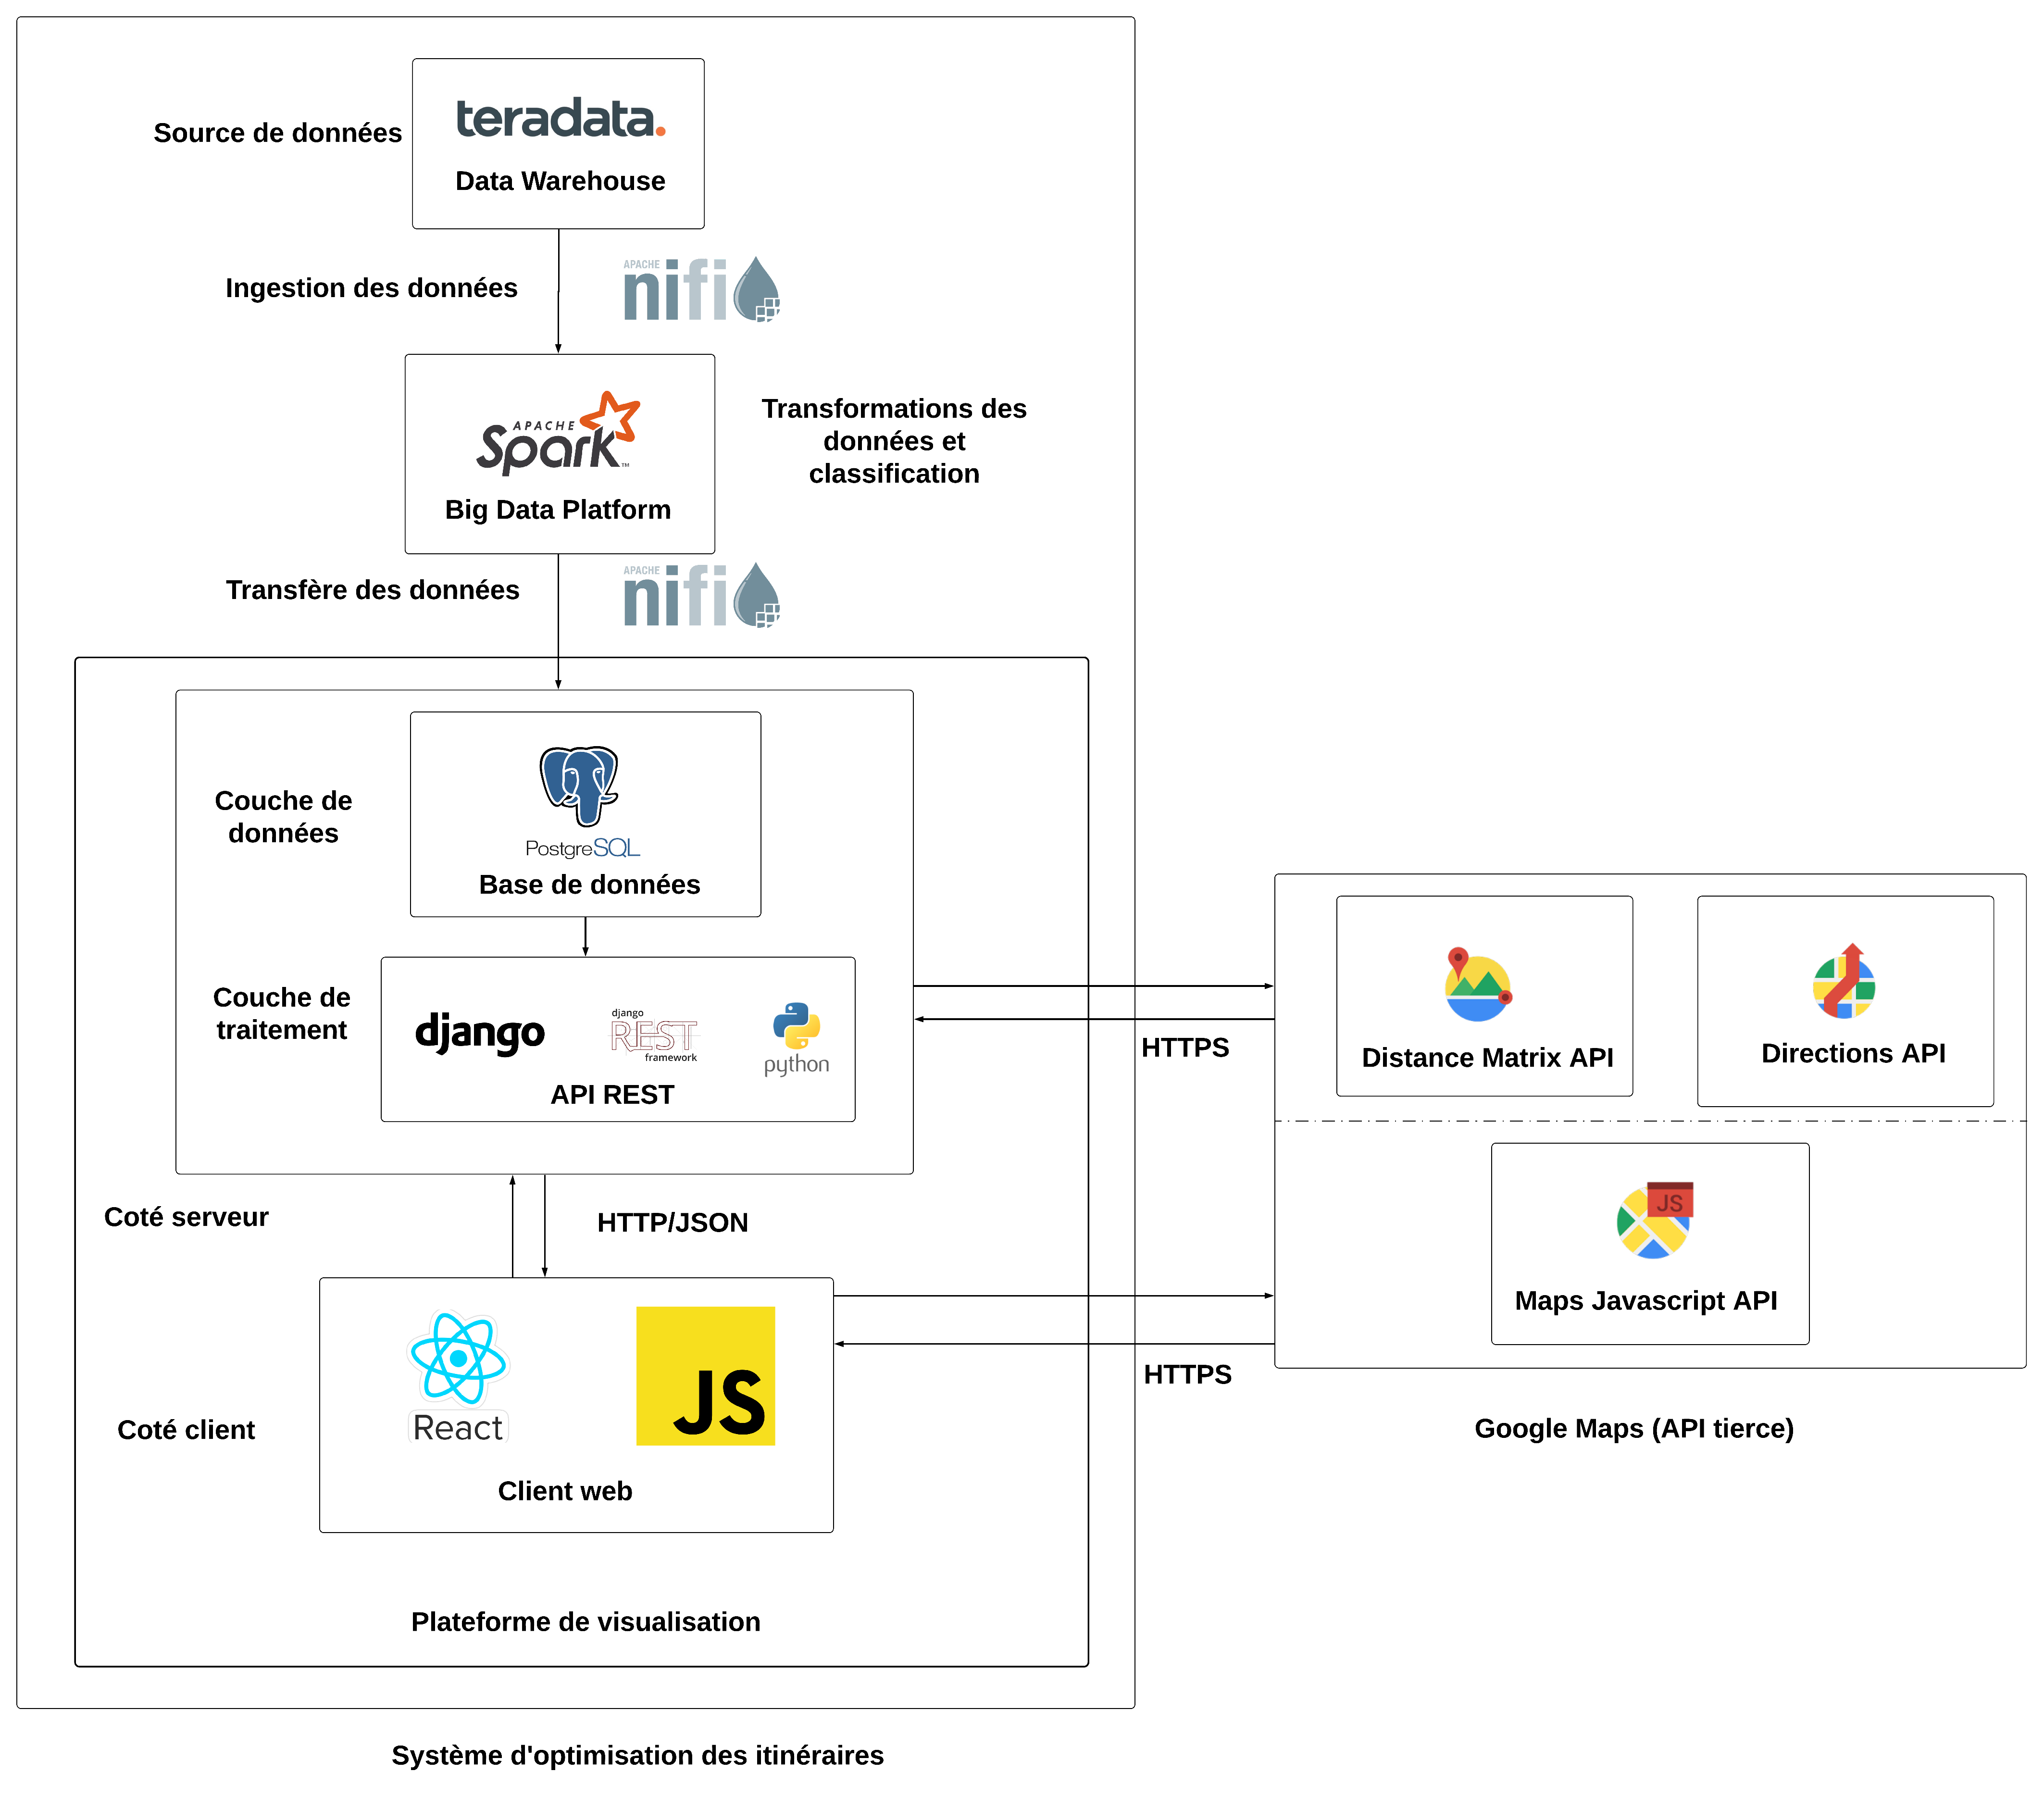
\includegraphics[height=15cm]{images_pfe/SYSTEM_ARCHITECTURE.png}
  \caption{Architecture technique de la solution.}
  \label{fig:technical-architecture}
\end{figure}
\FloatBarrier

La figure \ref{fig:technical-architecture} Lorem ipsum dolor sit amet, consectetur adipiscing elit. Proin posuere euismod neque, non semper nibh viverra sed. Praesent ut varius magna.Lorem ipsum dolor sit amet, consectetur adipiscing elit. Proin posuere euismod neque, non semper nibh viverra sed. Praesent ut varius magna. \textbf{Teradata Database} et il Lorem ipsum dolor sit amet, consectetur adipiscing elit. Proin posuere euismod neque, non semper nibh viverra sed. Praesent ut varius magna. \textbf{Apache Nifi} Lorem ipsum dolor sit amet, consectetur adipiscing elit. Proin posuere euismod neque, non semper nibh viverra sed. Praesent ut varius magna. \textbf{Apache Spark} via l'API Python \textbf{PySpark}. Lorem ipsum dolor sit amet, consectetur adipiscing elit. Proin posuere euismod neque, non semper nibh viverra sed. Praesent ut varius magna. \textbf{PostgreSQL} Lorem ipsum dolor sit amet, consectetur adipiscing elit. Proin posuere euismod neque, non semper nibh viverra sed. Praesent ut varius magna. \textbf{Django} sous le langage \textbf{Python}. Lorem ipsum dolor sit amet, consectetur adipiscing elit. Proin posuere euismod neque, non semper nibh viverra sed. Praesent ut varius magna. \textbf{Django Rest}. Le client web quant à lui, est implémenté avec la librairie \textbf{React.js} sous le langage \textbf{Javascript}. Le système communique avec les APIs \textbf{Google Maps} Lorem ipsum dolor sit amet, consectetur adipiscing elit. Proin posuere euismod neque, non semper nibh viverra sed. Praesent ut varius magna.I \textbf{Distance Matrix} Lorem ipsum dolor sit amet, consectetur adipiscing elit. Proin posuere euismod neque, non semper nibh viverra sed. Praesent ut varius magna. \textbf{Directions} Lorem ipsum dolor sit amet, consectetur adipiscing elit. Proin posuere euismod neque, non semper nibh viverra sed. Praesent ut varius magna.\textbf{Maps} Lorem ipsum dolor sit amet, consectetur adipiscing elit. Proin posuere euismod neque, non semper nibh viverra sed. Praesent ut varius magna.

\section{Technologies utilisées}

\subsection*{Teradata Database}

\begin{wrapfigure}{r}{0.3\textwidth}
  \centering
  
\includegraphics[width=0.28\textwidth]{images_pfe/Teradata_logo_2018.png}
  \caption{Logo de Teradata.}
\end{wrapfigure}
\FloatBarrier
Teradata Database \footnote{\url{https://www.teradata.com/} (visité le 11/08/2020).} Lorem ipsum dolor sit amet, consectetur adipiscing elit. Proin posuere euismod neque, non semper nibh viverra sed. Praesent ut varius magna. Fusce ipsum ante, semper nec interdum at, semper et lacus. Nulla ultrices magna a fringilla finibus. Etiam sollicitudin blandit ante. Vivamus blandit rhoncus tincidunt. Morbi sit amet congue purus. Praesent interdum gravida congue. Donec fermentum dui fermentum maximus rutrum.

\subsection*{Apache Nifi}
\begin{wrapfigure}{r}{0.3\textwidth}
  \centering
  
\includegraphics[width=0.2\textwidth]{images_pfe/apache_nifi_logo.png}
  \caption{Logo de Nifi.}
\end{wrapfigure}
\FloatBarrier
Apache Nifi \footnote{\url{https://nifi.apache.org/} (visité le 11/08/2020).} Lorem ipsum dolor sit amet, consectetur adipiscing elit. Proin posuere euismod neque, non semper nibh viverra sed. Praesent ut varius magna. Fusce ipsum ante, semper nec interdum at, semper et lacus. Nulla ultrices magna a fringilla finibus. Etiam sollicitudin blandit ante. Vivamus blandit rhoncus tincidunt. Morbi sit amet congue purus. Praesent interdum gravida congue. Donec fermentum dui fermentum maximus rutrum.


\subsection*{Apache Spark}
\begin{wrapfigure}{r}{0.3\textwidth}
  \centering
  
\includegraphics[width=0.28\textwidth]{images_pfe/Apache_Spark_logo.png}
  \caption{Logo de Spark.}
\end{wrapfigure}
\FloatBarrier
Apache Spark \footnote{\url{https://spark.apache.org/} (visité le 11/08/2020).} Lorem ipsum dolor sit amet, consectetur adipiscing elit. Proin posuere euismod neque, non semper nibh viverra sed. Praesent ut varius magna. (\textbf{PySpark}) Lorem ipsum dolor sit amet, consectetur adipiscing elit. Proin posuere euismod neque, non semper nibh viverra sed. Praesent ut varius magna. Fusce ipsum ante, semper nec interdum at, semper et lacus. Nulla ultrices magna a fringilla finibus. Etiam sollicitudin blandit ante. Vivamus blandit rhoncus tincidunt. Morbi sit amet congue purus. Praesent interdum gravida congue. Donec fermentum dui fermentum maximus rutrum.


\subsection*{PostgreSQL}
\begin{wrapfigure}[9]{r}{0.3\textwidth}
  \centering
  
\includegraphics[width=0.2\textwidth]{images_pfe/postgres_logo.png}
  \caption{Logo de PostgreSQL.}
\end{wrapfigure}
\FloatBarrier
PostgreSQL \footnote{\url{https://www.postgresql.org/} (visité le 11/08/2020).} Lorem ipsum dolor sit amet, consectetur adipiscing elit. Proin posuere euismod neque, non semper nibh viverra sed. Praesent ut varius magna. Fusce ipsum ante, semper nec interdum at, semper et lacus. Nulla ultrices magna a fringilla finibus. Etiam sollicitudin blandit ante. Vivamus blandit rhoncus tincidunt. Morbi sit amet congue purus. Praesent interdum gravida congue. Donec fermentum dui fermentum maximus rutrum.


\subsection*{Python}

\begin{wrapfigure}[6]{r}{0.3\textwidth}
  \centering
  
\includegraphics[width=0.12\textwidth]{images_pfe/python_logo.png}
  \caption{Logo de Python.}
\end{wrapfigure}
\FloatBarrier
Python \footnote{\url{https://www.python.org/} (visité le 11/08/2020).} Lorem ipsum dolor sit amet, consectetur adipiscing elit. Proin posuere euismod neque, non semper nibh viverra sed. Praesent ut varius magna. Fusce ipsum ante, semper nec interdum at, semper et lacus. Nulla ultrices magna a fringilla finibus. Etiam sollicitudin blandit ante. Vivamus blandit rhoncus tincidunt. Morbi sit amet congue purus.

\vspace{.5cm}

\subsection*{Django}

\begin{wrapfigure}{r}{0.3\textwidth}
  \centering
  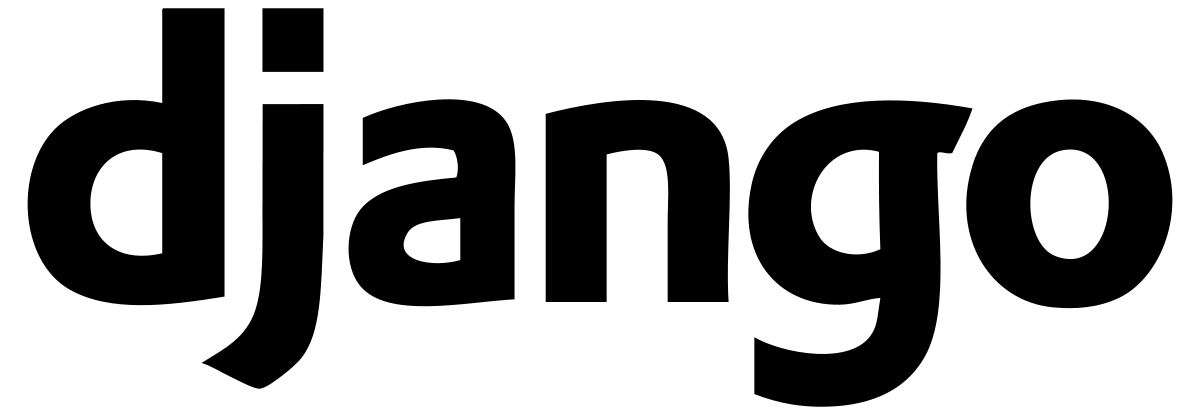
\includegraphics[width=0.2\textwidth]{images_pfe/django_logo.png}
  \caption{Logo de Django.}
\end{wrapfigure}
\FloatBarrier
Django \footnote{\url{https://www.djangoproject.com/} (visité le 11/08/2020).} Lorem ipsum dolor sit amet, consectetur adipiscing elit. Proin posuere euismod neque, non semper nibh viverra sed. Praesent ut varius magna. Fusce ipsum ante, semper nec interdum at, semper et lacus. Nulla ultrices magna a fringilla finibus. Etiam sollicitudin blandit ante. Vivamus blandit rhoncus tincidunt. Morbi sit amet congue purus. Praesent interdum gravida congue. Donec fermentum dui fermentum maximus rutrum.

\vspace{.5cm}

\subsection*{Django Rest Framework}

\begin{wrapfigure}{r}{0.3\textwidth}
  \centering
  
\includegraphics[width=0.25\textwidth]{images_pfe/django_rest.png}
  \caption{Logo de Django Rest Framework.}
\end{wrapfigure}
\FloatBarrier
Django REST \footnote{\url{https://www.django-rest-framework.org/} (visité le 11/08/2020).}Lorem ipsum dolor sit amet, consectetur adipiscing elit. Proin posuere euismod neque, non semper nibh viverra sed. Praesent ut varius magna. Fusce ipsum ante, semper nec interdum at, semper et lacus. Nulla ultrices magna a fringilla finibus. Etiam sollicitudin blandit ante. Vivamus blandit rhoncus tincidunt. Morbi sit amet congue purus. Praesent interdum gravida congue. Donec fermentum dui fermentum maximus rutrum.

\vspace{.5cm}

\subsection*{Javascript}
\begin{wrapfigure}[6]{r}{0.3\textwidth}
  \centering
  
\includegraphics[width=0.2\textwidth]{images_pfe/js_logo.png}
  \caption{Logo de Javascript.}
\end{wrapfigure}
\FloatBarrier
JavaScript \footnote{\url{https://developer.mozilla.org/fr/docs/Web/JavaScript} (visité le 11/08/2020).} Lorem ipsum dolor sit amet, consectetur adipiscing elit. Proin posuere euismod neque, non semper nibh viverra sed. Praesent ut varius magna. Fusce ipsum ante, semper nec interdum at, semper et lacus. Nulla ultrices magna a fringilla finibus. Etiam sollicitudin blandit ante. Vivamus blandit rhoncus tincidunt. Morbi sit amet congue purus. Praesent interdum gravida congue. 

\vspace{3cm}

\subsection*{React.js}

\begin{wrapfigure}[6]{r}{0.3\textwidth}
  \centering
  
\includegraphics[width=0.2\textwidth]{images_pfe/react_logo.png}
  \caption{Logo de React.js.}
\end{wrapfigure}
\FloatBarrier
React.js \footnote{\url{https://fr.reactjs.org/} (visité le 12/08/2020).} Lorem ipsum dolor sit amet, consectetur adipiscing elit. Proin posuere euismod neque, non semper nibh viverra sed. Praesent ut varius magna. Fusce ipsum ante, semper nec interdum at, semper et lacus. Nulla ultrices magna a fringilla finibus. Etiam sollicitudin blandit ante. Vivamus blandit rhoncus tincidunt. Morbi sit amet congue purus. 

\vspace{1cm}

\subsection*{Distance Matrix API}
\begin{wrapfigure}[6]{r}{0.3\textwidth}
  \centering
  
\includegraphics[width=0.2\textwidth]{images_pfe/google_distance_matrix_api.png}
  \caption{Logo de l'API Distance Matrix.}
\end{wrapfigure}
\FloatBarrier
L'API Distance Matrix \footnote{\url{https://developers.google.com/maps/documentation/distance-matrix/overview} (visité le 12/08/2020).} Lorem ipsum dolor sit amet, consectetur adipiscing elit. Proin posuere euismod neque, non semper nibh viverra sed. Praesent ut varius magna. Fusce ipsum ante, semper nec interdum at, semper et lacus. Nulla ultrices magna a fringilla finibus. Etiam sollicitudin blandit ante. Vivamus blandit rhoncus tincidunt. Morbi sit amet congue purus. 

\vspace{1cm}

\subsection*{Directions API}
\begin{wrapfigure}[6]{r}{0.3\textwidth}
  \centering
  
\includegraphics[width=0.2\textwidth]{images_pfe/google_directions_api.png}
  \caption{Logo de l'API Directions.}
\end{wrapfigure}
\FloatBarrier
L'API Directions \footnote{\url{https://developers.google.com/maps/documentation/directions/overview} (visité le 12/08/2020).} Lorem ipsum dolor sit amet, consectetur adipiscing elit. Proin posuere euismod neque, non semper nibh viverra sed. Praesent ut varius magna. Fusce ipsum ante, semper nec interdum at, semper et lacus. Nulla ultrices magna a fringilla finibus. Etiam sollicitudin blandit ante. Vivamus blandit rhoncus tincidunt. Morbi sit amet congue purus. 

\vspace{1cm}

\subsection*{Maps Javascript API}
\begin{wrapfigure}[6]{r}{0.3\textwidth}
  \centering
  
\includegraphics[width=0.2\textwidth]{images_pfe/google_maps_js.png}
  \caption{Logo de l'API Maps Javascript.}
\end{wrapfigure}
\FloatBarrier
L'API Maps JavaScript \footnote{\url{https://developers.google.com/maps/documentation/javascript/overview} (visité le 12/08/2020).} Lorem ipsum dolor sit amet, consectetur adipiscing elit. Proin posuere euismod neque, non semper nibh viverra sed. Praesent ut varius magna. Fusce ipsum ante, semper nec interdum at, semper et lacus. Nulla ultrices magna a fringilla finibus. Etiam sollicitudin blandit ante. Vivamus blandit rhoncus tincidunt. Morbi sit amet congue purus. Praesent interdum gravida congue. 

\vspace{1cm}

\section{Conclusion}
Lorem ipsum dolor sit amet, consectetur adipiscing elit. Proin posuere euismod neque, non semper nibh viverra sed. Praesent ut varius magna. Fusce ipsum ante, semper nec interdum at, semper et lacus. Nulla ultrices magna a fringilla finibus. Etiam sollicitudin blandit ante. Vivamus blandit rhoncus tincidunt. Morbi sit amet congue purus. Praesent interdum gravida congue. Donec fermentum dui fermentum maximus rutrum.














\chapter{Tests et résultats}
\clearpage
\section{Introduction}
Lorem ipsum dolor sit amet, consectetur adipiscing elit. Proin posuere euismod neque, non semper nibh viverra sed. Praesent ut varius magna. Fusce ipsum ante, semper nec interdum at, semper et lacus. Nulla ultrices magna a fringilla finibus. Etiam sollicitudin blandit ante. Vivamus blandit rhoncus tincidunt. Morbi sit amet congue purus. Praesent interdum gravida congue. Donec fermentum dui fermentum maximus rutrum.


\subsection{Analyse des variables}
L'objectif de l'analyse des variables (Voir annexe \ref{app:initial-dataset}) était d'identifier les relations et les corrélations contenues dans les données. Pour cela nous avons utilisé deux méthodes : la matrice de corrélation (Voir figure \ref{fig:all-features-correlations}) et la matrice de puissance prédictive (Voir figure \ref{fig:all-features-pps}). La matrice de corrélation contient les coefficients de corrélation entre chaque paire de variable (Voir annexe \ref{app:correlation}). 

\begin{figure}[hbt!]
  \centering
  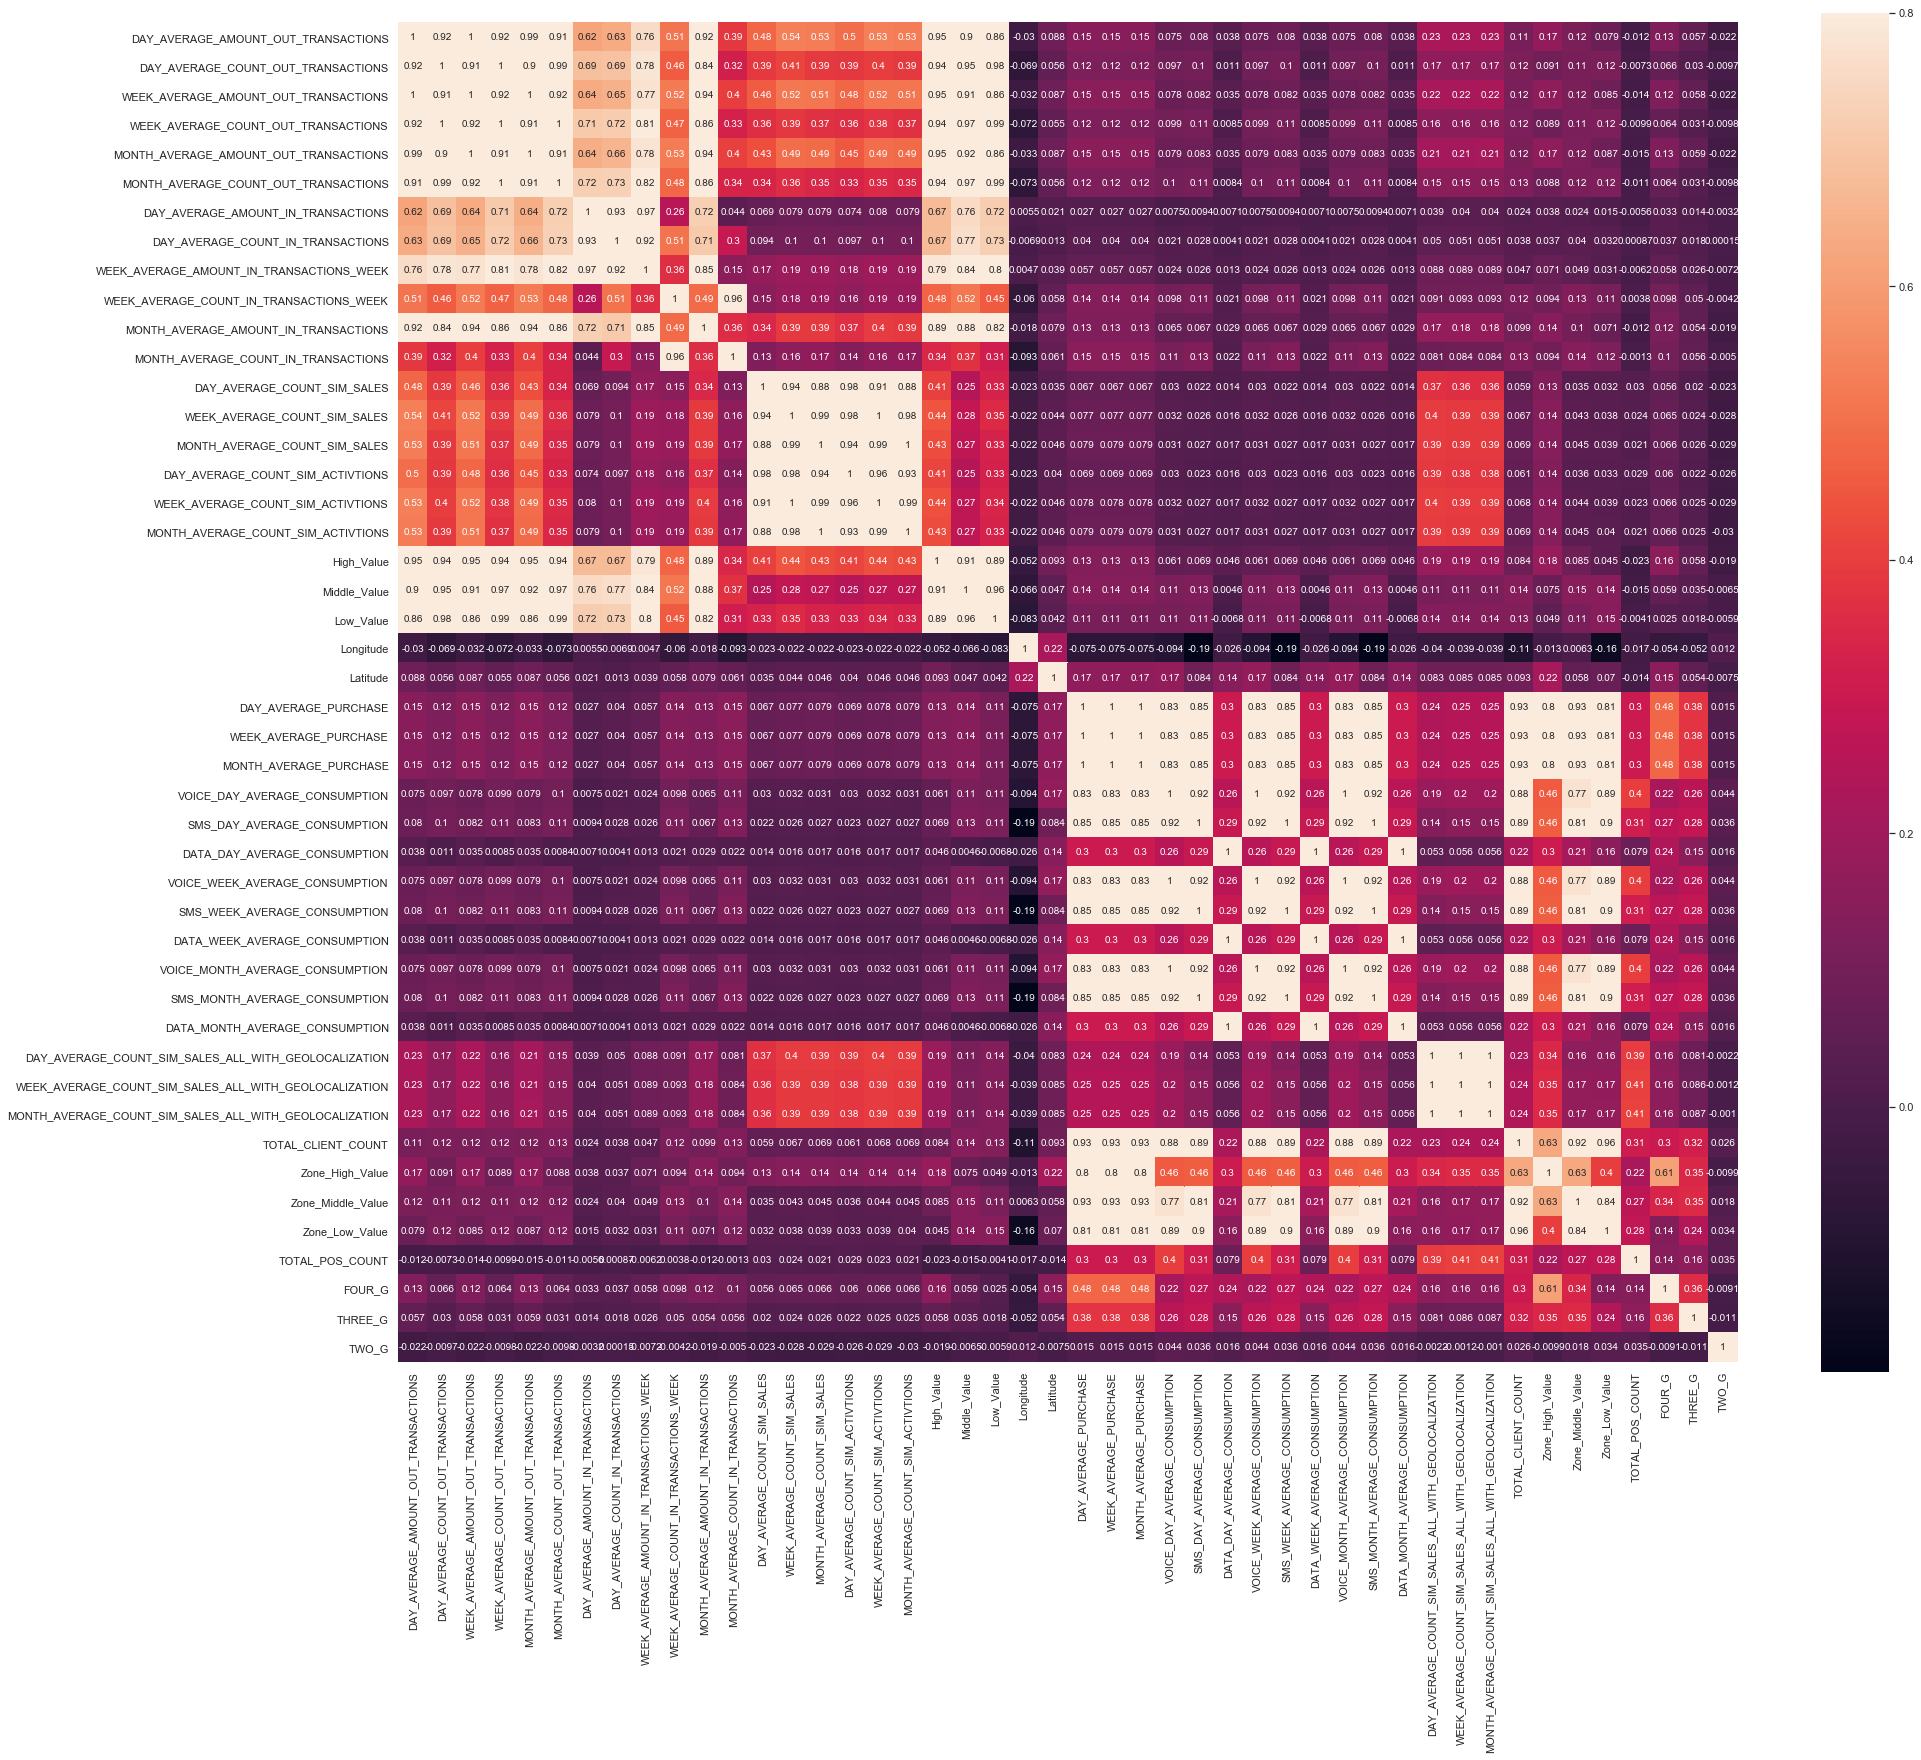
\includegraphics[width=12cm]{images_pfe/features_correlations.png}
  \caption{Matrice de corrélation (les couleurs claires désignent une forte corrélation).}
  \label{fig:all-features-correlations}
\end{figure}
\FloatBarrier

Lorem ipsum dolor sit amet, consectetur adipiscing elit. Proin posuere euismod neque, non semper nibh viverra sed. Praesent ut varius magna. Fusce ipsum ante, semper nec interdum at, semper et lacus. Nulla ultrices magna a fringilla finibus. Etiam sollicitudin blandit ante. Vivamus blandit rhoncus tincidunt. Morbi sit amet congue purus. Praesent interdum gravida congue. Donec fermentum dui fermentum maximus rutrum. Le score de puissance de prédiction entre une variable $X$ et une variable $Y$ représente la précision avec validation croisée du modèle contenant la variable $X$ seulement pour prédire la variable $Y$. Lorem ipsum dolor sit amet, consectetur adipiscing elit. Proin posuere euismod neque, non semper nibh viverra sed. Praesent ut varius magna. Fusce ipsum ante, semper nec interdum at, semper et lacus. Nulla ultrices magna a fringilla finibus. Etiam sollicitudin blandit ante. Vivamus blandit rhoncus tincidunt. Morbi sit amet congue purus. Praesent interdum gravida congue. Donec fermentum dui fermentum maximus rutrum. \parencite{wetschoreck_rip_2020}.

\begin{figure}[hbt!]
  \centering
  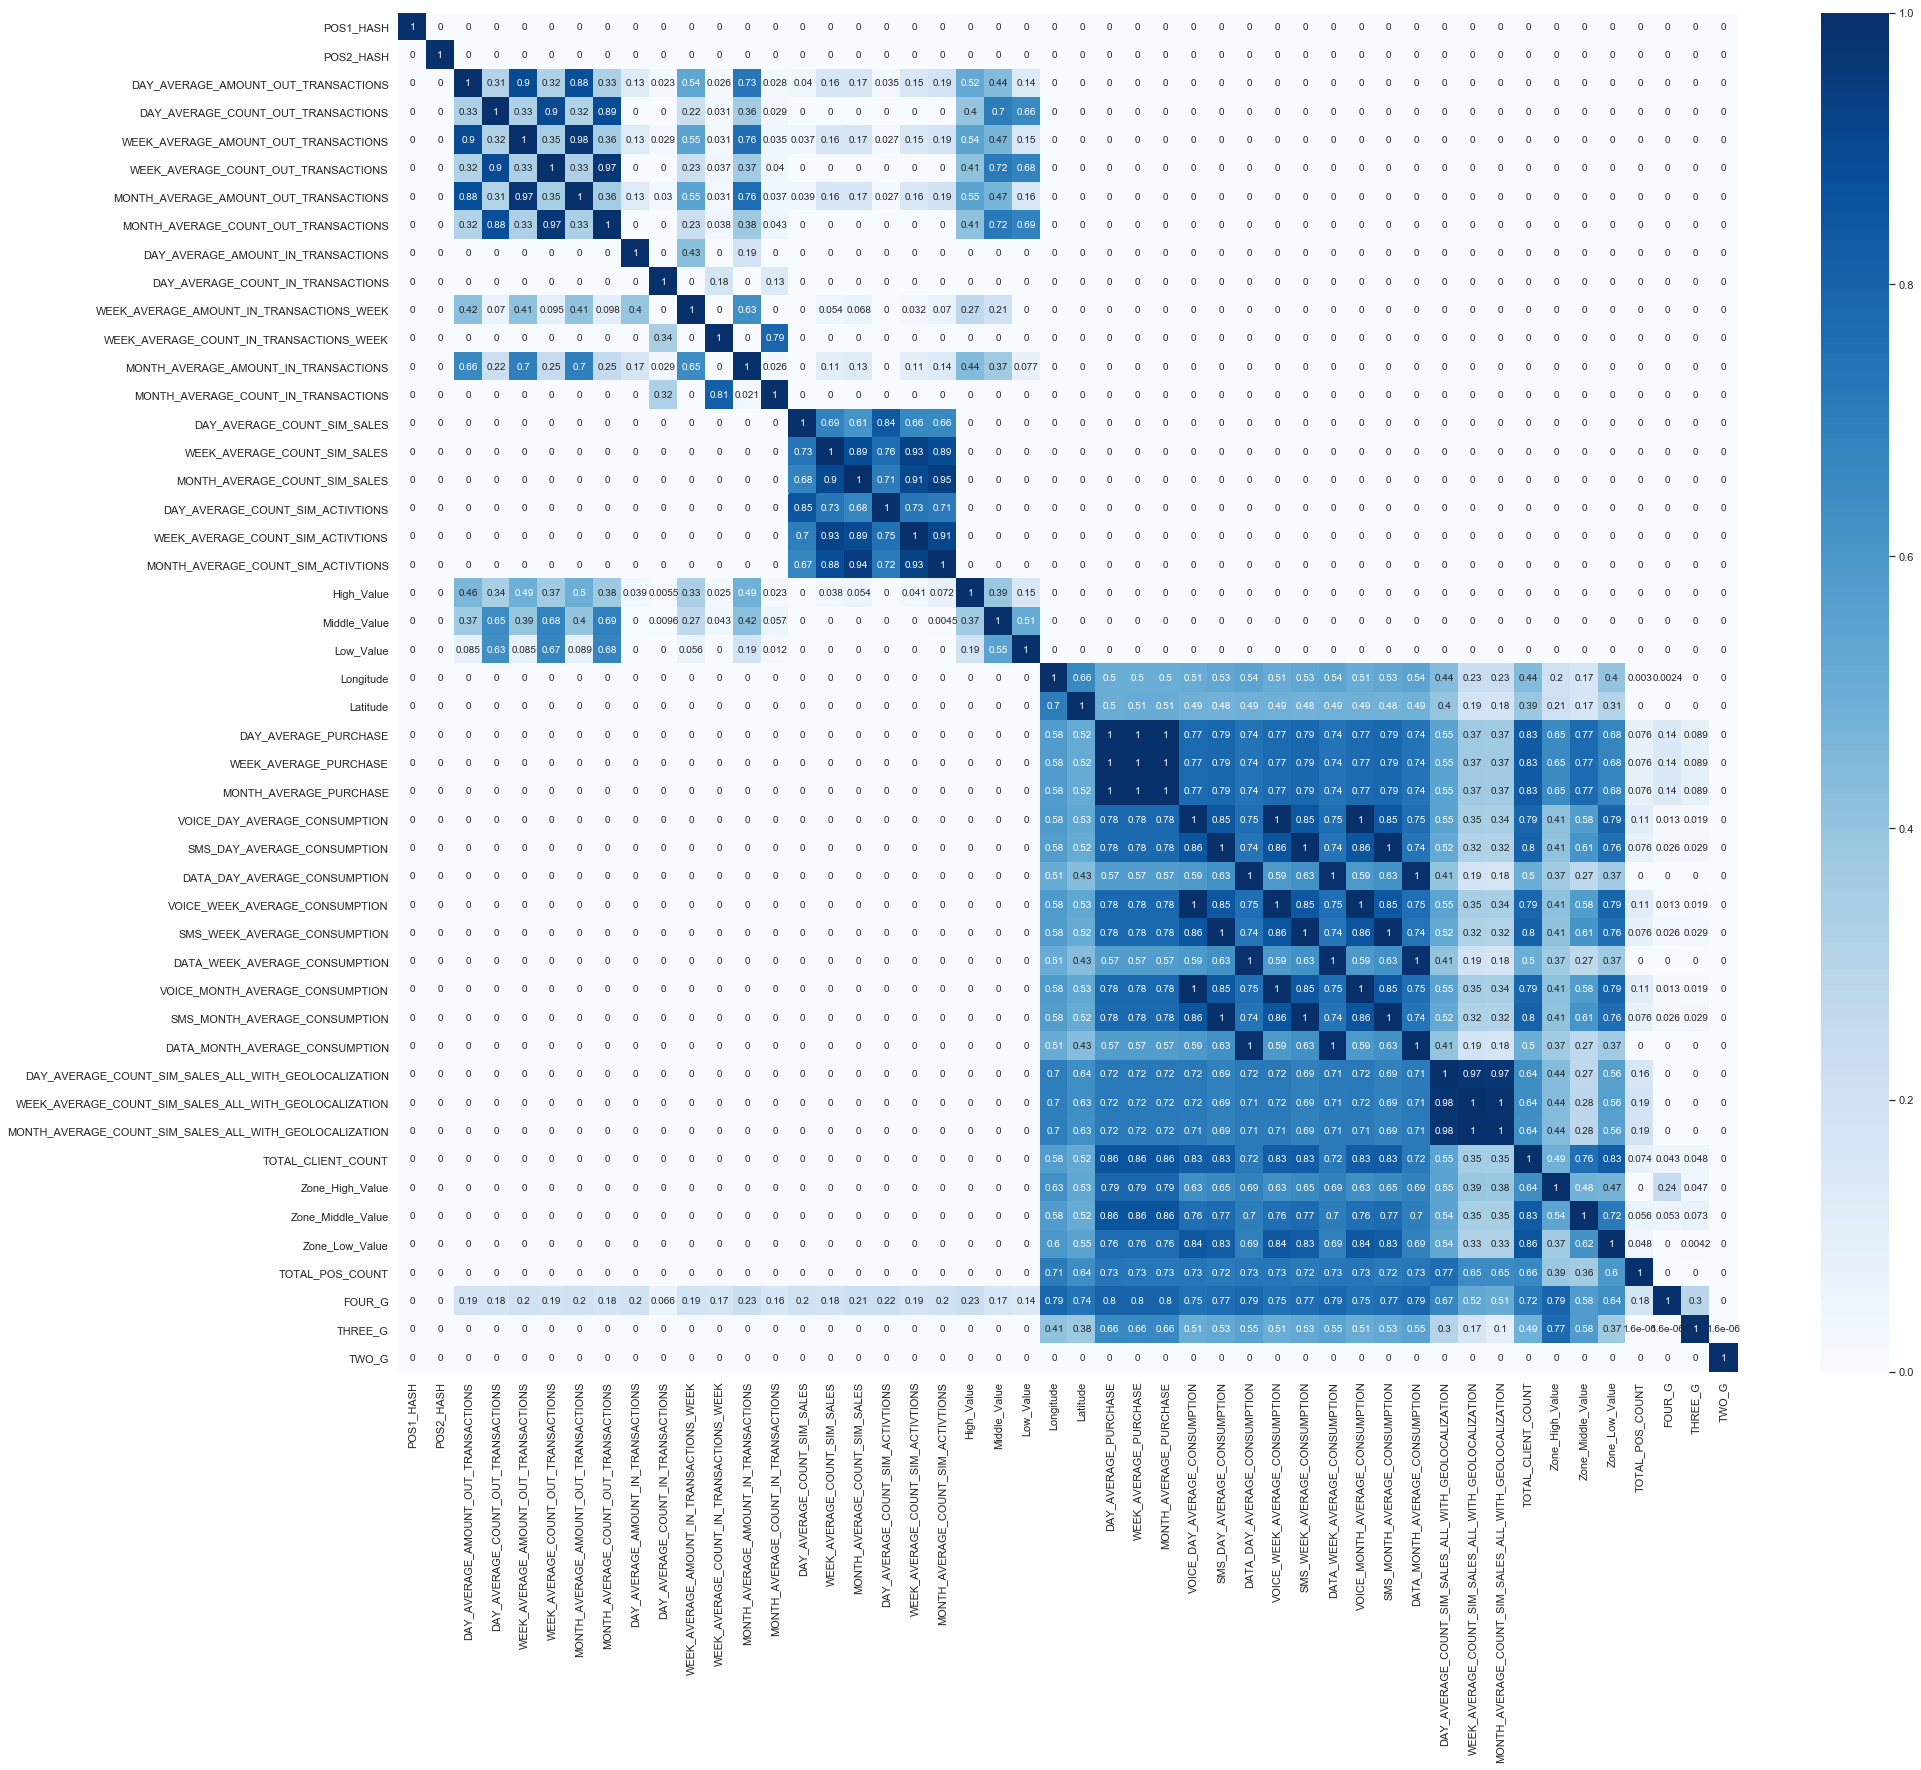
\includegraphics[width=12cm]{images_pfe/features_pps.png}
  \caption{Matrice de puissance de prédiction (les couleurs foncées désignent une forte puissance de prédiction).}
  \label{fig:all-features-pps}
\end{figure}
\FloatBarrier

La première remarque que nous tirons de la matrice de corrélation (figure \ref{fig:all-features-correlations}) Lorem ipsum dolor sit amet, consectetur adipiscing elit. Proin posuere euismod neque, non semper nibh viverra sed. Praesent ut varius magna. Fusce ipsum ante, semper nec interdum at, semper et lacus. Nulla ultrices magna a fringilla finibus. Etiam sollicitudin blandit ante. Vivamus blandit rhoncus tincidunt. Morbi sit amet congue purus. Praesent interdum gravida congue. Donec fermentum dui fermentum maximus rutrum. (Voir annexe \ref{app:initial-dataset}).Lorem ipsum dolor sit amet, consectetur adipiscing elit. Proin posuere euismod neque, non semper nibh viverra sed. Praesent ut varius magna. Fusce ipsum ante, semper nec interdum at, semper et lacus. Nulla ultrices magna a fringilla finibus. Etiam sollicitudin blandit ante. Vivamus blandit rhoncus tincidunt. Morbi sit amet congue purus. Praesent interdum gravida congue. Donec fermentum dui fermentum maximus rutrum.

\medskip

Lorem ipsum dolor sit amet, consectetur adipiscing elit. Proin posuere euismod neque, non semper nibh viverra sed. Praesent ut varius magna. Fusce ipsum ante, semper nec interdum at, semper et lacus. Nulla ultrices magna a fringilla finibus. Etiam sollicitudin blandit ante. Vivamus blandit rhoncus tincidunt. Morbi sit amet congue purus. Praesent interdum gravida congue. Donec fermentum dui fermentum maximus rutrum.

\medskip

Les figures \ref{fig:chosen-features-correlations} Lorem ipsum dolor sit amet, consectetur adipiscing elit. Proin posuere euismod neque, non semper nibh viverra sed. Praesent ut varius magna. Fusce ipsum ante, semper nec interdum at, semper et lacus. Nulla ultrices magna a fringilla finibus. Etiam sollicitudin blandit ante. Vivamus blandit rhoncus tincidunt. Morbi sit amet congue purus. Praesent interdum gravida congue. Donec fermentum dui fermentum maximus rutrum. : \\

\begin{figure}[hbt!]
  \begin{subfigure}[t]{0.4\textwidth}
  \centering
  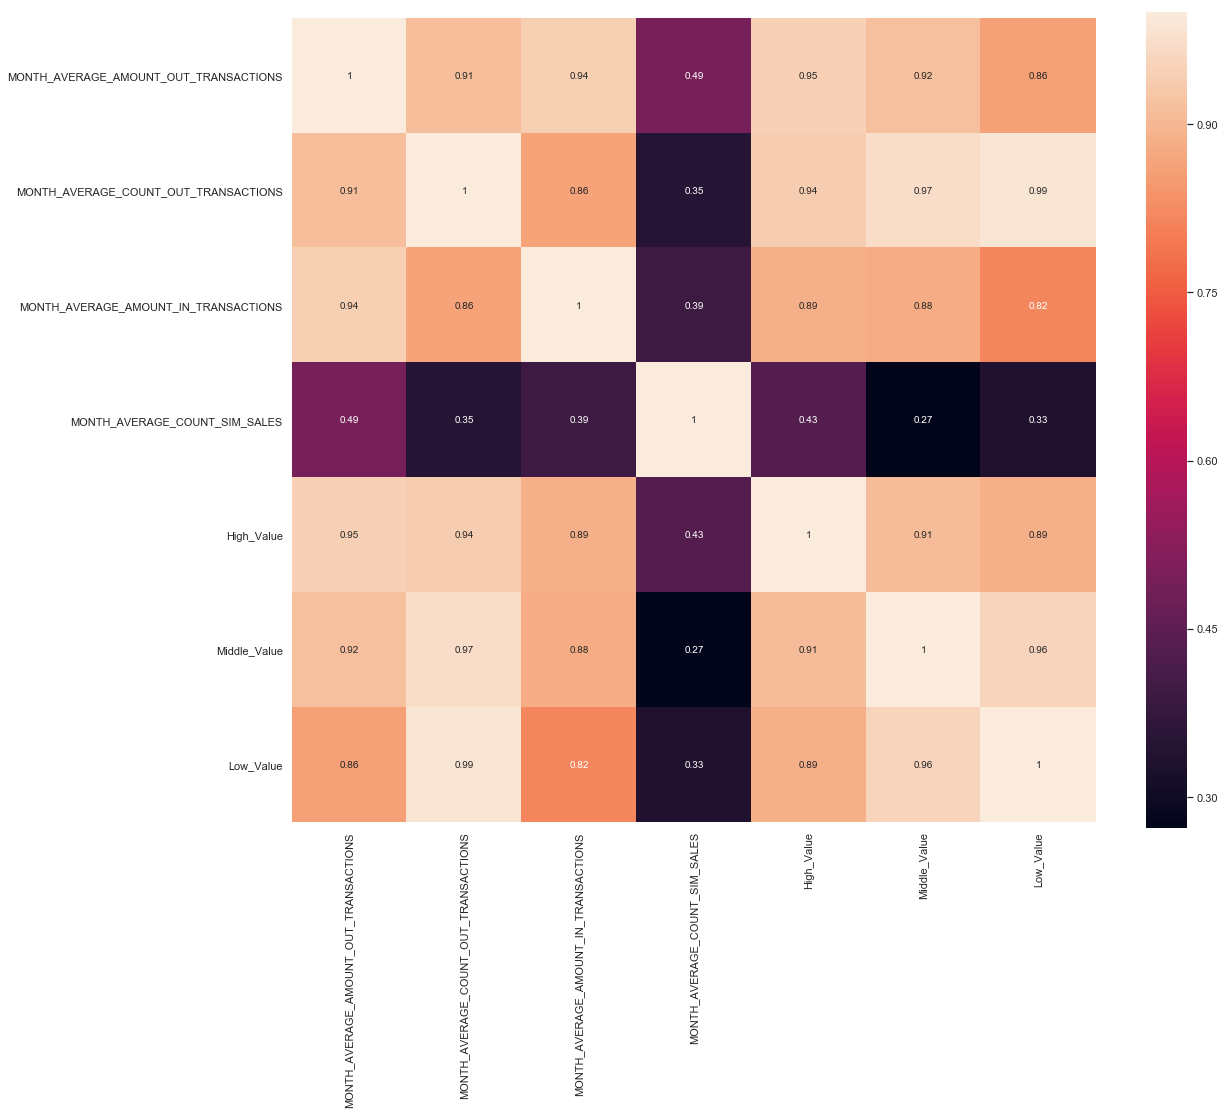
\includegraphics[width=\linewidth]{images_pfe/feature_correlations.png}
  \caption{Matrice de corrélation des variable sélectionnées.}
  \label{fig:chosen-features-correlations}
  \end{subfigure}\hfill
  \begin{subfigure}[t]{0.4\textwidth}
  \centering
  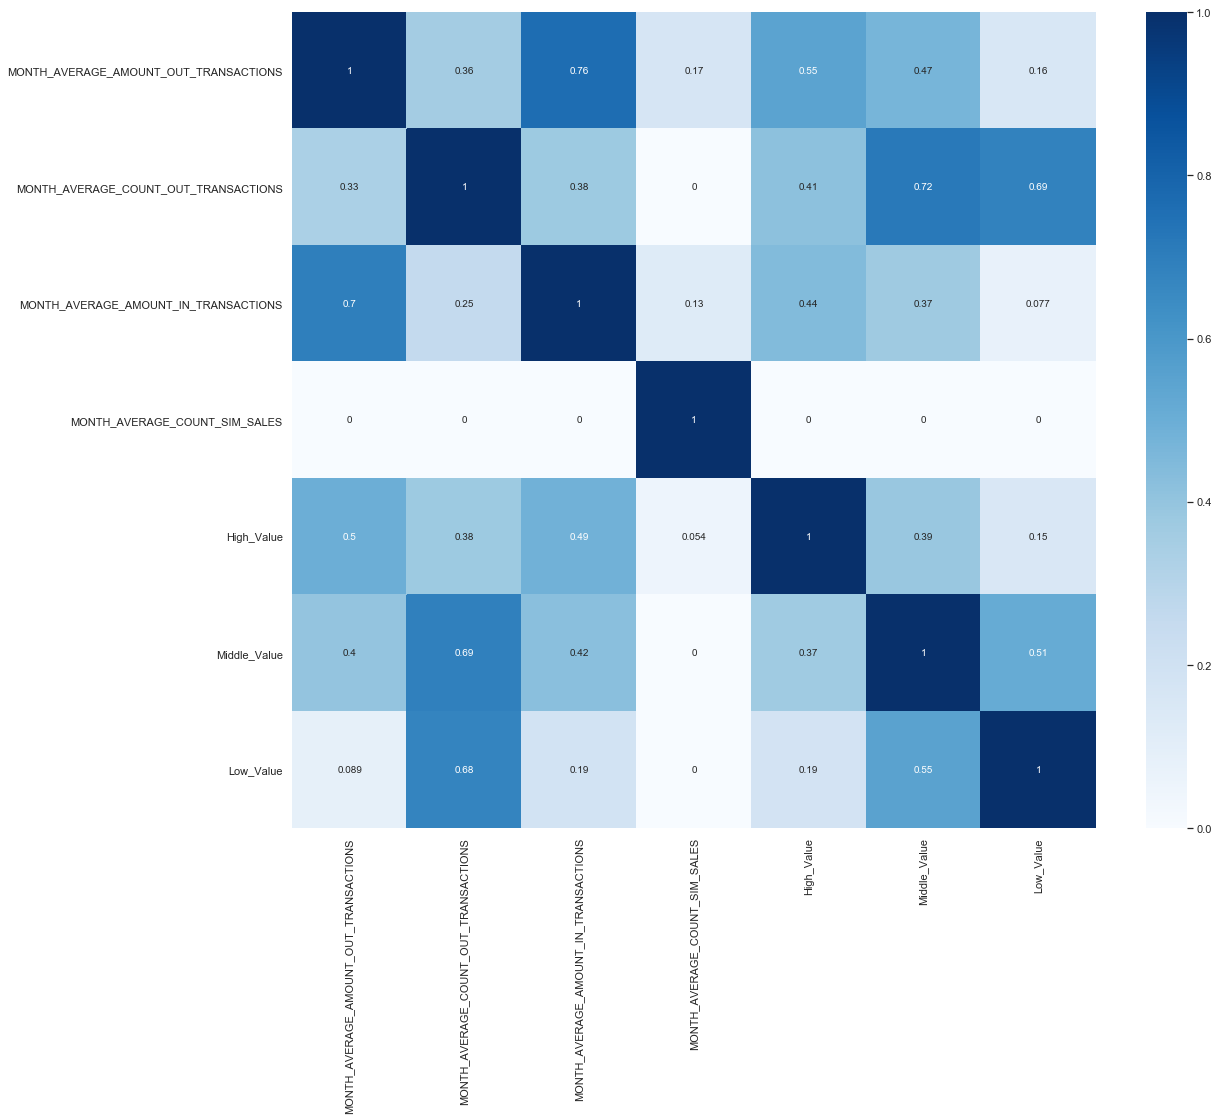
\includegraphics[width=\linewidth]{images_pfe/features_pps2.png}
  \caption{Matrice de puissance de prédiction des variables sélectionnées.}
  \label{fig:chosen-features-pps}
  \end{subfigure}
\end{figure}
\FloatBarrier


\subsection{Clustering}
Lorem ipsum dolor sit amet, consectetur adipiscing elit. Proin posuere euismod neque, non semper nibh viverra sed. Praesent ut varius magna. Fusce ipsum ante, semper nec interdum at, semper et lacus. Nulla ultrices magna a fringilla finibus. Etiam sollicitudin blandit ante. Vivamus blandit rhoncus tincidunt. Morbi sit amet congue purus. Praesent interdum gravida congue. Donec fermentum dui fermentum maximus rutrum.

\medskip

La première méthode était le clustering hiérarchique (Voir annexe \ref{app:hierarchical-clustering}). Lorem ipsum dolor sit amet, consectetur adipiscing elit. Proin posuere euismod neque, non semper nibh viverra sed. Praesent ut varius magna. Fusce ipsum ante, semper nec interdum at, semper et lacus. Nulla ultrices magna a fringilla finibus. Etiam sollicitudin blandit ante. Vivamus blandit rhoncus tincidunt. Morbi sit amet congue purus. Praesent interdum gravida congue. Donec fermentum dui fermentum maximus rutrum..

\begin{figure}[hbt!]
  \centering
  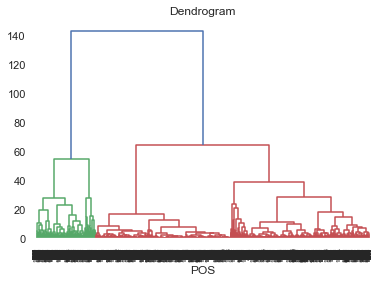
\includegraphics[width=10cm]{images_pfe/hirarchichal_clustering.png}
  \caption{Dendrogramme du clustering hiérarchique.}
  \label{fig:hierarchical-clustering}
\end{figure}
\FloatBarrier

La figure \ref{fig:hierarchical-clustering} Lorem ipsum dolor sit amet, consectetur adipiscing elit. Proin posuere euismod neque, non semper nibh viverra sed. Praesent ut varius magna. Fusce ipsum ante, semper nec interdum at, semper et lacus. Nulla ultrices magna a fringilla finibus. Etiam sollicitudin blandit ante. Vivamus blandit rhoncus tincidunt. Morbi sit amet congue purus. Praesent interdum gravida congue. Donec fermentum dui fermentum maximus rutrum. \ref{app:k-means}) Lorem ipsum dolor sit amet, consectetur adipiscing elit. Proin posuere euismod neque, non semper nibh viverra sed. Praesent ut varius magna. 

\medskip

Lorem ipsum dolor sit amet, consectetur adipiscing elit. Proin posuere euismod neque, non semper nibh viverra sed. Praesent ut varius magna. Fusce ipsum ante, semper nec interdum at, semper et lacus. Nulla ultrices magna a fringilla finibus. Etiam sollicitudin blandit ante. Vivamus blandit rhoncus tincidunt. Morbi sit amet congue purus. Praesent interdum gravida congue. Donec fermentum dui fermentum maximus rutrum. $K$ Lorem ipsum dolor sit amet, consectetur adipiscing elit. Proin posuere euismod neque, non semper nibh viverra sed. Praesent ut varius magna. Fusce ipsum ante, semper nec interdum at, semper et lacus. Nulla ultrices magna a fringilla finibus. Etiam sollicitudin blandit ante. Vivamus blandit rhoncus tincidunt. Morbi sit amet congue purus. Praesent interdum gravida congue. Donec fermentum dui fermentum maximus rutrum. \parencite{kassambara_determining_nodate}.

\begin{figure}[hbt!]
  \centering
  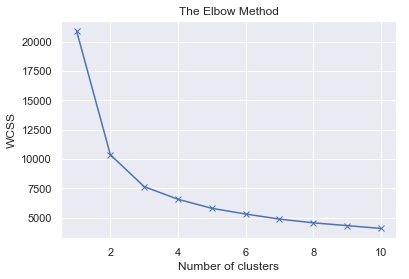
\includegraphics[width=10cm]{images_pfe/elbow_method.png}
  \caption{Résultat de la méthode Elbow.}
  \label{fig:elbow-method}
\end{figure}
\FloatBarrier

La figure \ref{fig:elbow-method}Lorem ipsum dolor sit amet, consectetur adipiscing elit. Proin posuere euismod neque, non semper nibh viverra sed. Praesent ut varius magna. Fusce ipsum ante, semper nec interdum at, semper et lacus. Nulla ultrices magna a fringilla finibus. Etiam sollicitudin blandit ante. Vivamus blandit rhoncus tincidunt. Morbi sit amet congue purus. Praesent interdum gravida congue. Donec fermentum dui fermentum maximus rutrum. $K$ valant 2 ou 3. Lorem ipsum dolor sit amet, consectetur adipiscing elit. Proin posuere euismod neque, non semper nibh viverra sed. Praesent ut varius magna. 

\medskip

Lorem ipsum dolor sit amet, consectetur adipiscing elit. Proin posuere euismod neque, non semper nibh viverra sed. Praesent ut varius magna. Fusce ipsum ante, semper nec interdum at, semper et lacus. Nulla ultrices magna a fringilla finibus. Etiam sollicitudin blandit ante. Vivamus blandit rhoncus tincidunt. Morbi sit amet congue purus. Praesent interdum gravida congue. Donec fermentum dui fermentum maximus rutrum.Lorem ipsum dolor sit amet, consectetur adipiscing elit. Proin posuere euismod neque, non semper nibh viverra sed. Praesent ut varius magna. Fusce ipsum ante, semper nec interdum at, semper et lacus. \parencite{kassambara_determining_nodate}.

\begin{figure}[hbt!]
  \centering
  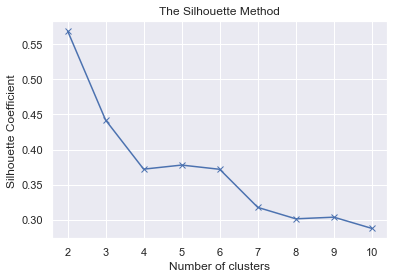
\includegraphics[width=10cm]{images_pfe/silhouette.png}
  \caption{Résultat de la méthode Silhouette.}
  \label{fig:silhouette-method}
\end{figure}
\FloatBarrier

La figure \ref{fig:silhouette-method} Lorem ipsum dolor sit amet, consectetur adipiscing elit. Proin posuere euismod neque, non semper nibh viverra sed. Praesent ut varius magna. Fusce ipsum ante, semper nec interdum at, semper et lacus. Nulla ultrices magna a fringilla finibus. Etiam sollicitudin blandit ante. Vivamus blandit rhoncus tincidunt. Morbi sit amet congue purus. Praesent interdum gravida congue. Donec fermentum dui fermentum maximus rutrum. $K = 2$ et ça rejoint le résultats de la méthode Elbow.

\medskip

Lorem ipsum dolor sit amet, consectetur adipiscing elit. Proin posuere euismod neque, non semper nibh viverra sed. Praesent ut varius magna.(Voir annexe \ref{app:pca}) Lorem ipsum dolor sit amet, consectetur adipiscing elit. Proin posuere euismod neque, non semper nibh viverra sed. Praesent ut varius magna.s (Voir annexe \ref{app:final-dataset}) . Lorem ipsum dolor sit amet, consectetur adipiscing elit. Proin posuere euismod neque, non semper nibh viverra sed. Praesent ut varius magna. (Voir figure \ref{fig:pca-method}). Les variables Lorem ipsum dolor sit amet, consectetur adipiscing elit. Nam massa magna, vulputate non sem eu, faucibus venenatis enim. Nullam sit amet pretium enim, sit amet condimentum magna. Mauris at pulvinar quam. Curabitur tincidunt tellus mi, auctor sodales nibh porttitor at. Aenean lobortis consequat aliquet. Suspendisse commodo euismod urna, eu finibus eros ultrices at. Donec ut dui nunc. Etiam ultrices ullamcorper ligula, ac tristique sapien scelerisque et. Donec sapien augue, vestibulum sit amet accumsan vel, varius eu odio.(Voir figure \ref{fig:correlation-circle}).


\begin{figure}[hbt!]
  \centering
  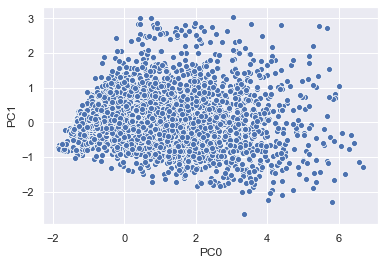
\includegraphics[width=10cm]{images_pfe/pca_results.png}
  \caption{Résultat de l'analyse en composantes principales.}
  \label{fig:pca-method}
\end{figure}
\FloatBarrier


Lorem ipsum dolor sit amet, consectetur adipiscing elit. Proin posuere euismod neque, non semper nibh viverra sed. Praesent ut varius magna. Fusce ipsum ante, semper nec interdum at, semper et lacus. Nulla ultrices magna a fringilla finibus. Etiam sollicitudin blandit ante. Vivamus blandit rhoncus tincidunt. Morbi sit amet congue purus. Praesent interdum gravida congue. Donec fermentum dui fermentum maximus rutrum. La figure \ref{fig:kmeans-pca}Lorem ipsum dolor sit amet, consectetur adipiscing elit. Proin posuere euismod neque, non semper nibh viverra sed. Praesent ut varius magna. Fusce ipsum ante, semper nec interdum at, semper et lacus. Nulla ultrices magna a fringilla finibus. Etiam sollicitudin blandit ante. Vivamus blandit rhoncus tincidunt. Morbi sit amet congue purus. Praesent interdum gravida congue. Donec fermentum dui fermentum maximus rutrum.

\begin{figure}[hbt!]
  \centering
  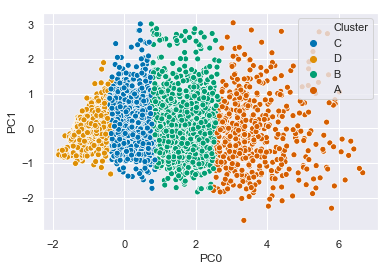
\includegraphics[width=10cm]{images_pfe/kmeans_clustering.png}
  \caption{Résultats de l'algorithme K-means en 2D (le cluster A en orange, B en vert, C en bleu et D en jaune).}
  \label{fig:kmeans-pca}
\end{figure}
\FloatBarrier

\subsection{Classification}
Lorem ipsum dolor sit amet, consectetur adipiscing elit. Proin posuere euismod neque, non semper nibh viverra sed. Praesent ut varius magna. Fusce ipsum ante, semper nec interdum at, semper et lacus. Nulla ultrices magna a fringilla finibus. Etiam sollicitudin blandit ante. Vivamus blandit rhoncus tincidunt. Morbi sit amet congue purus. Praesent interdum gravida congue. Donec fermentum dui fermentum maximus rutrum. (Voir les annexes \ref{app:random-forest}, \ref{app:svm}, \ref{app:naive-bays} et \ref{app:xgboost}). Pour évaluer ces différents algorithme nous avons utilisé le score $\text{F}_1$ moyen de toutes les classes (A, B, C et D). Le score $\text{F}_1$ est une mesure de la qualité de classification avec un score idéal égal à 1 . Le calcul du score $\text{F}_1$ d'une classe donnée se fait comme suit :
\begin{equation*}
    \text{F}_1 = 2 × \frac{\text{précision} ×  \text{rappel}}{\text{précision}+\text{rappel}}
\end{equation*}
avec :
\begin{equation*}
    \text{précision} = \frac{\text{Vrais positifs}}{\text{Vrais positifs}+\text{Faux positifs}}
\end{equation*}
et 
\begin{equation*}
    \text{rappel} = \frac{\text{Vrais positifs}}{\text{Vrais positifs}+\text{Faux négatifs}}
\end{equation*}

Un résultat est positif si sa classe prédite est la classe positive (ex: A), négatif sinon (ex: B, C ou D). Il est vrai si sa classe prédite correspond à sa classe réelle, faux sinon.


\begin{table}[h!]
    \centering
    \begin{tabular}{|c|c|c|}
        \hline
        Algorithme & score $\text{F}_1$ moyen  & score $\text{F}_1$ moyen avec validation croisée \\
        \hline
         Random Forest & 0.97 &  0.96 \\
        \hline
         SVM & 0.99 & 0.98 \\
        \hline
        Naive Bays & 0.94 &  0.94 \\
        \hline
        XGBoost & 0.98 &  0.97\\
        \hline
    \end{tabular}
    \caption{Évaluation des différents algorithmes de classification.}
    \label{tab:f1-scores}
\end{table}
\FloatBarrier


Le tableau \ref{tab:f1-scores} Lorem ipsum dolor sit amet, consectetur adipiscing elit. Proin posuere euismod neque, non semper nibh viverra sed. Praesent ut varius magna. Fusce ipsum ante, semper nec interdum at, semper et lacus. Nulla ultrices magna a fringilla finibus. Etiam sollicitudin blandit ante. Vivamus blandit rhoncus tincidunt. Morbi sit amet congue purus. Praesent interdum gravida congue. Donec fermentum dui fermentum maximus rutrum.

\subsection{Élaboration des plans de visite}
Lorem ipsum dolor sit amet, consectetur adipiscing elit. Proin posuere euismod neque, non semper nibh viverra sed. Praesent ut varius magna. Fusce ipsum ante, semper nec interdum at, semper et lacus. Nulla ultrices magna a fringilla finibus. Etiam sollicitudin blandit ante. Vivamus blandit rhoncus tincidunt. Morbi sit amet congue purus. Praesent interdum gravida congue. Donec fermentum dui fermentum maximus rutrum. (Voir \ref{tab:ptsp-results-comparison}). Le tableau ci-dessous illustre les différents résultats.


\begin{xltabular}{12cm}{|X|X|X|}
    \hline
    Instance & Notre algorithme     & MSC      \\\hline
    p01      &  440.94  & \textbf{432.10}   \\\hline
    p02      & 1118.70 & \textbf{1105.81}  \\\hline
    p03      & 494.45  & \textbf{466.71}   \\\hline
    p04      & 589.61  & \textbf{549.05}   \\\hline
    p05      & 1398.54 & \textbf{1382.33}  \\\hline
    p06      & 693.08  & \textbf{643.50}   \\\hline
    p07      & 670.34  & \textbf{643.80}   \\\hline
    p08      & 1645.90 & \textbf{1611.96}  \\\hline
    p09      & 838.06  & \textbf{720.72}   \\\hline
    p10      & 1310.29 & \textbf{1233.53}  \\\hline
    p11      & \textbf{490.95}& 490.97   \\\hline
    p12      & \textbf{664.07}  & 664.10   \\\hline
    p13      & 831.30  & \textbf{830.80}   \\\hline
    p14      & 996.86  & \textbf{994.60}   \\\hline
    p15      & 1159.94 & \textbf{1157.07}  \\\hline
    p16      & 664.21  & \textbf{649.96}   \\\hline
    p17      & 786.24  & \textbf{774.54}   \\\hline
    p18      & 886.94  & \textbf{873.73}   \\\hline
    p19      & 974.44  & \textbf{958.51}   \\\hline
    p20      & 1062.35 & \textbf{1033.58}  \\\hline
    p21      & \textbf{1374.88} & 1375.07 \\\hline
    p22      & 4321.96 & \textbf{4312.31}  \\\hline
    p23      & 8517.44 & \textbf{8308.48}  \\\hline
    pr01     & \textbf{2064.74} & 2064.84  \\\hline
    pr02     & 3220.29 & \textbf{3205.94}  \\\hline
    pr03     & 4065.70 & \textbf{4027.71}  \\\hline
    pr04     & 4609.59 & \textbf{4538.19}  \\\hline
    pr05     & 4706.05 & \textbf{4613.58}  \\\hline
    pr06     & 5633.53 & \textbf{5521.24}  \\\hline
    pr07     & 4472.17 & \textbf{4435.39}  \\\hline
    pr08     & 5457.90 & \textbf{5366.53}  \\\hline
    pr09     & 7352.93 & \textbf{7234.35}  \\\hline
    pr10     & 8360.00 & \textbf{8199.55}  \\\hline
    Diff \%  & 2.43    &    \\\hline 
    \caption{Comparaison entre les résultats de notre algorithme d'optimisation avec les meilleures solutions connues du PTSP}
    \label{tab:ptsp-final-results-comparison}
\end{xltabular}
\FloatBarrier

\medskip
Le tableau \ref{tab:ptsp-final-results-comparison} Lorem ipsum dolor sit amet, consectetur adipiscing elit. Proin posuere euismod neque, non semper nibh viverra sed. Praesent ut varius magna. Fusce ipsum ante, semper nec interdum at, semper et lacus. Nulla ultrices magna a fringilla finibus. Etiam sollicitudin blandit ante. Vivamus blandit rhoncus tincidunt. Morbi sit amet congue purus. Praesent interdum gravida congue. Donec fermentum dui fermentum maximus rutrum.

\medskip
Lorem ipsum dolor sit amet, consectetur adipiscing elit. Proin posuere euismod neque, non semper nibh viverra sed. Praesent ut varius magna. Fusce ipsum ante, semper nec interdum at, semper et lacus. Nulla ultrices magna a fringilla finibus. Etiam sollicitudin blandit ante. Vivamus blandit rhoncus tincidunt. Morbi sit amet congue purus. Praesent interdum gravida congue. Donec fermentum dui fermentum maximus rutrum. \parencite{noauthor_route_2020}. Lorem ipsum dolor sit amet, consectetur adipiscing elit. Proin posuere euismod neque, non semper nibh viverra sed. Praesent ut varius magna. Fusce ipsum ante, semper nec interdum at, semper et lacus. Nulla ultrices magna a fringilla finibus. Etiam sollicitudin blandit ante. Vivamus blandit rhoncus tincidunt. Morbi sit amet congue purus. Praesent interdum gravida congue. Donec fermentum dui fermentum maximus rutrum.




\subsection{Le dataflow Nifi}
Le but du dataflow Nifi est d'orchestrer et d'établir le lien entre les différentes parties du système. La figure \ref{fig:nifi-dataflow} Lorem ipsum dolor sit amet, consectetur adipiscing elit. Proin posuere euismod neque, non semper nibh viverra sed. Praesent ut varius magna. Fusce ipsum ante, semper nec interdum at, semper et lacus. Nulla ultrices magna a fringilla finibus. Etiam sollicitudin blandit ante. Vivamus blandit rhoncus tincidunt. Morbi sit amet congue purus. Praesent interdum gravida congue. Donec fermentum dui fermentum maximus rutrum.

\begin{figure}[hbt!]
  \centering
  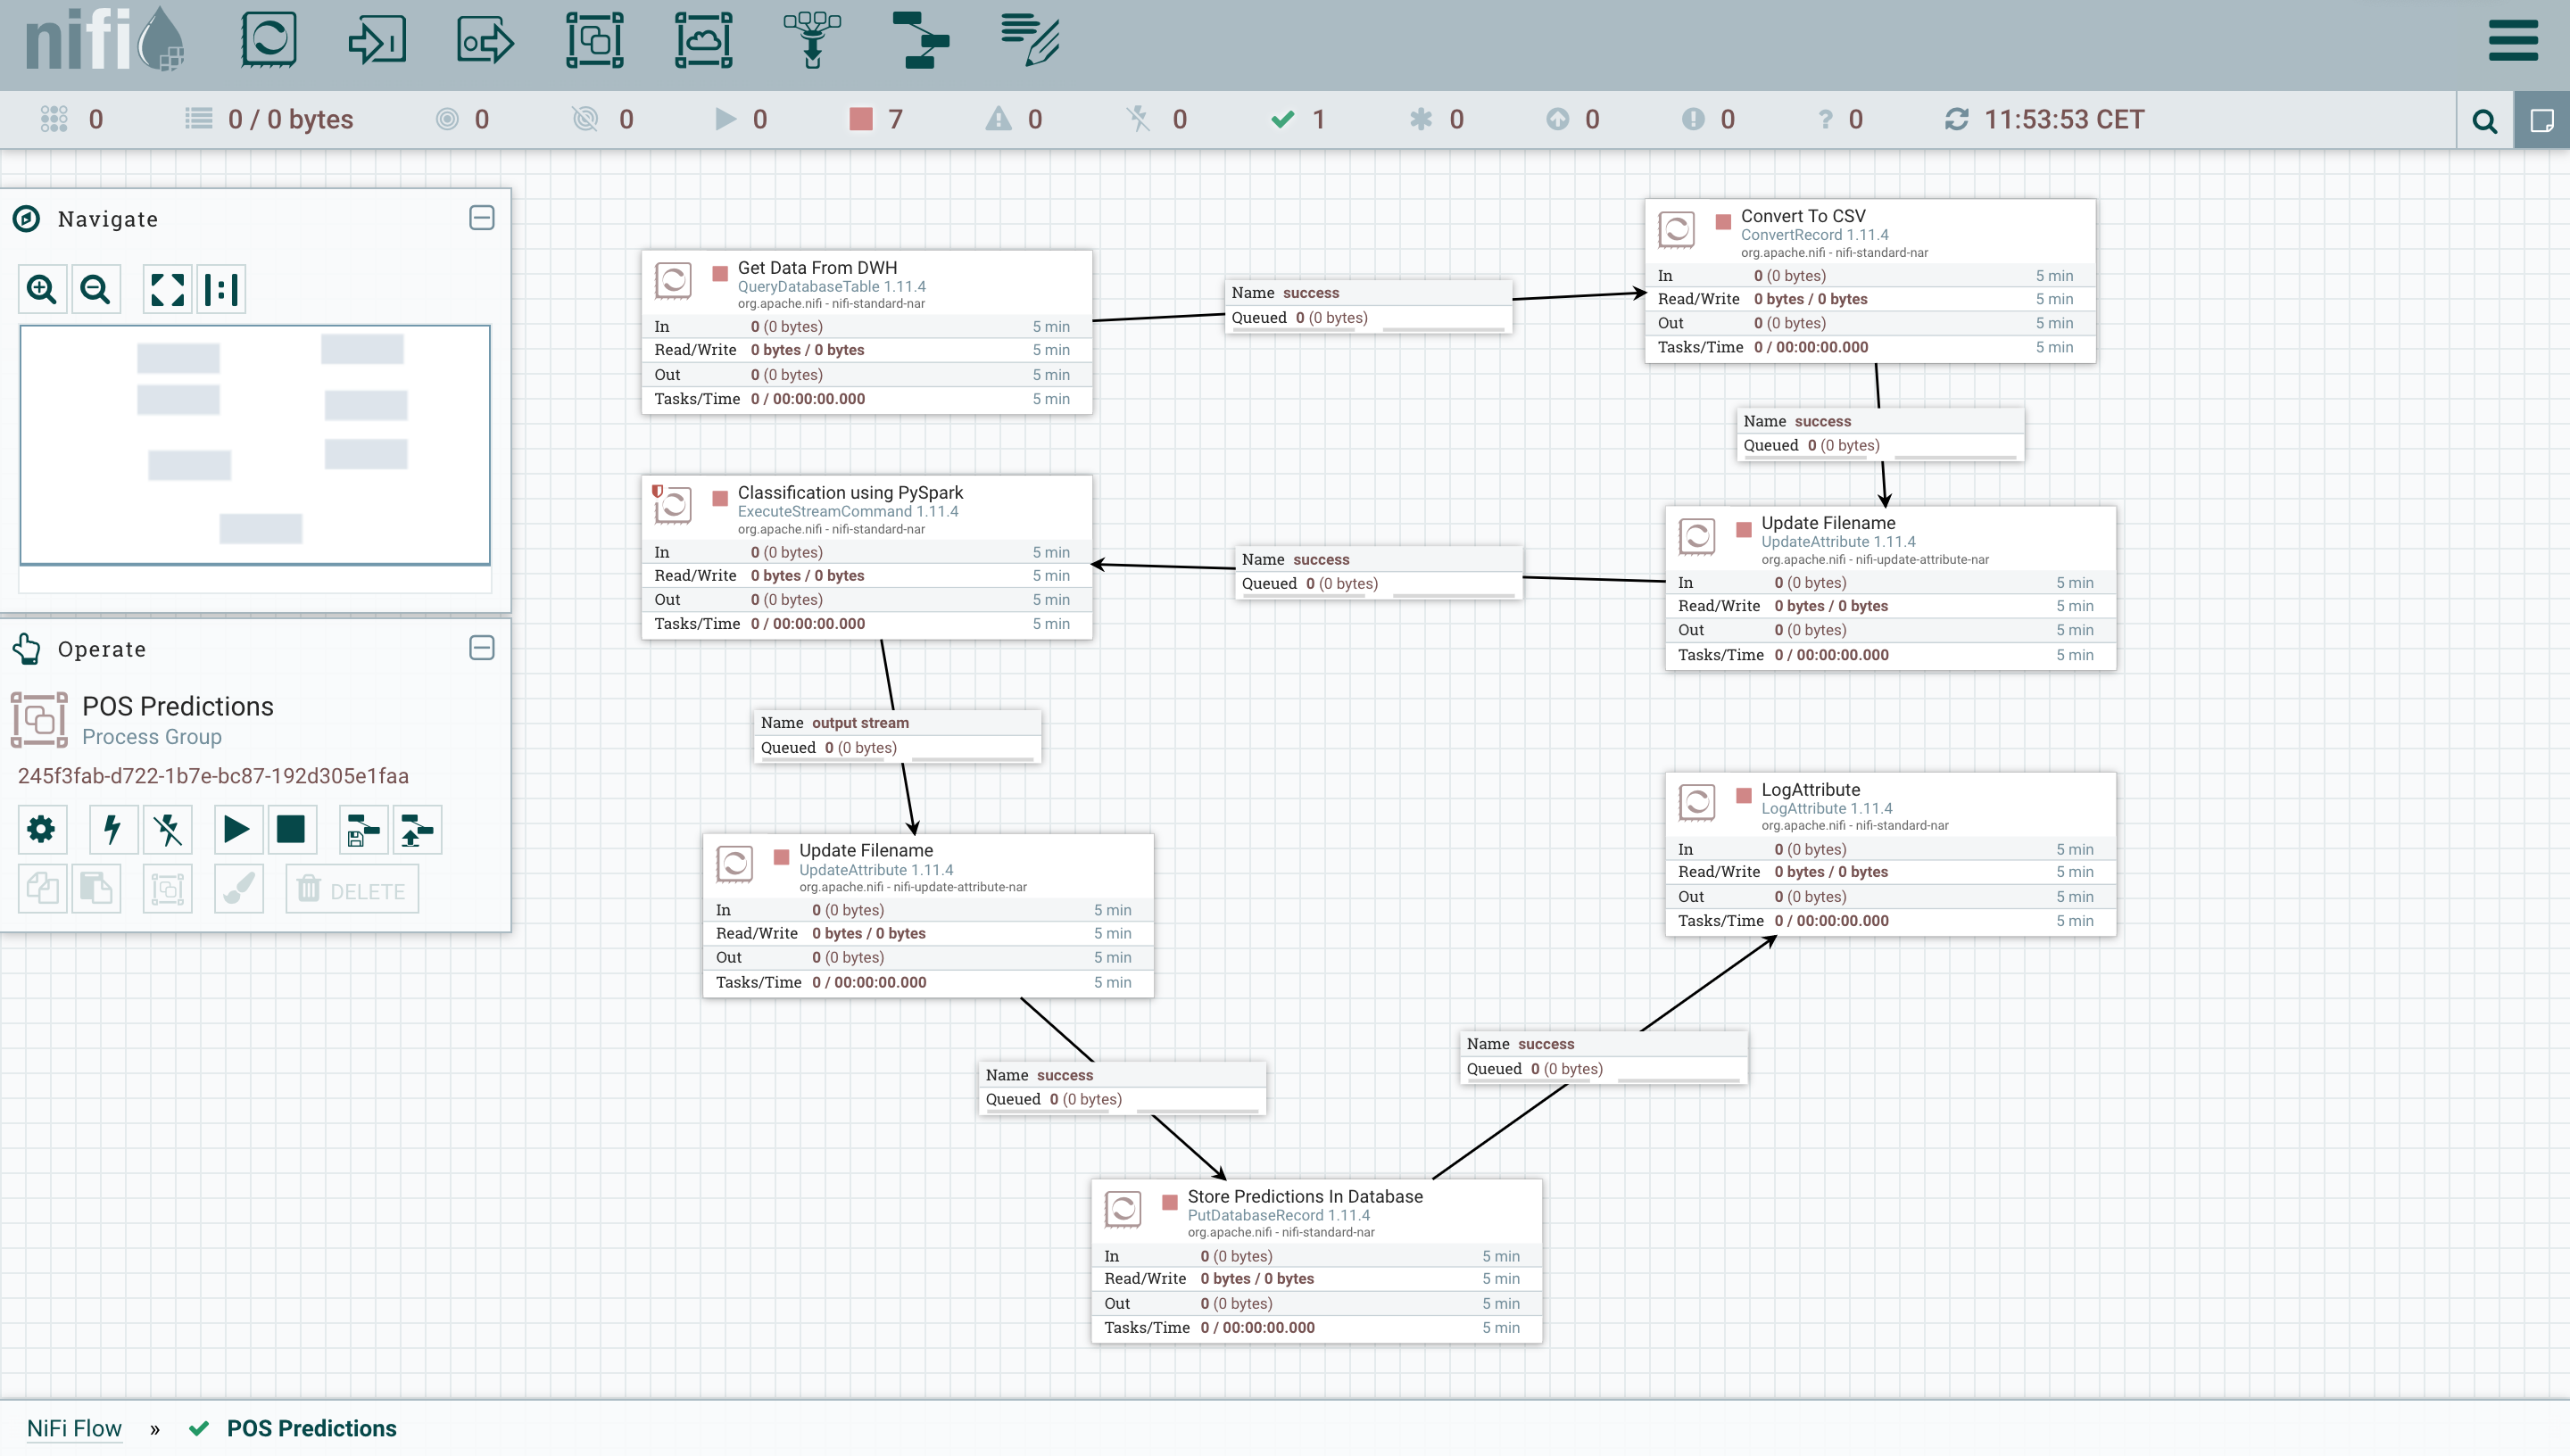
\includegraphics[width=15cm]{images_pfe/NIFI_DATAFLOW.png}
  \caption{Dataflow Nifi.}
  \label{fig:nifi-dataflow}
\end{figure}
\FloatBarrier

\subsection{La plateforme de visualisation}
Lorem ipsum dolor sit amet, consectetur adipiscing elit. Proin posuere euismod neque, non semper nibh viverra sed. Praesent ut varius magna. Fusce ipsum ante, semper nec interdum at, semper et lacus. Nulla ultrices magna a fringilla finibus. Etiam sollicitudin blandit ante. Vivamus blandit rhoncus tincidunt. Morbi sit amet congue purus. Praesent interdum gravida congue. Donec fermentum dui fermentum maximus rutrum.

\medskip

Dans la page principale de la plateforme, nous retrouvons le tableau de bord (Voir figure \ref{fig:dashboard-page}). Lorem ipsum dolor sit amet, consectetur adipiscing elit. Proin posuere euismod neque, non semper nibh viverra sed. Praesent ut varius magna. Fusce ipsum ante, semper nec interdum at, semper et lacus. Nulla ultrices magna a fringilla finibus. Etiam sollicitudin blandit ante. Vivamus blandit rhoncus tincidunt. Morbi sit amet congue purus. Praesent interdum gravida congue. Donec fermentum dui fermentum maximus rutrum. \textit{POS} sous l'anglet \textit{Maps} (Voir figure \ref{fig:pos-page}). 

\medskip



\begin{figure}[hbt!]
  \centering
  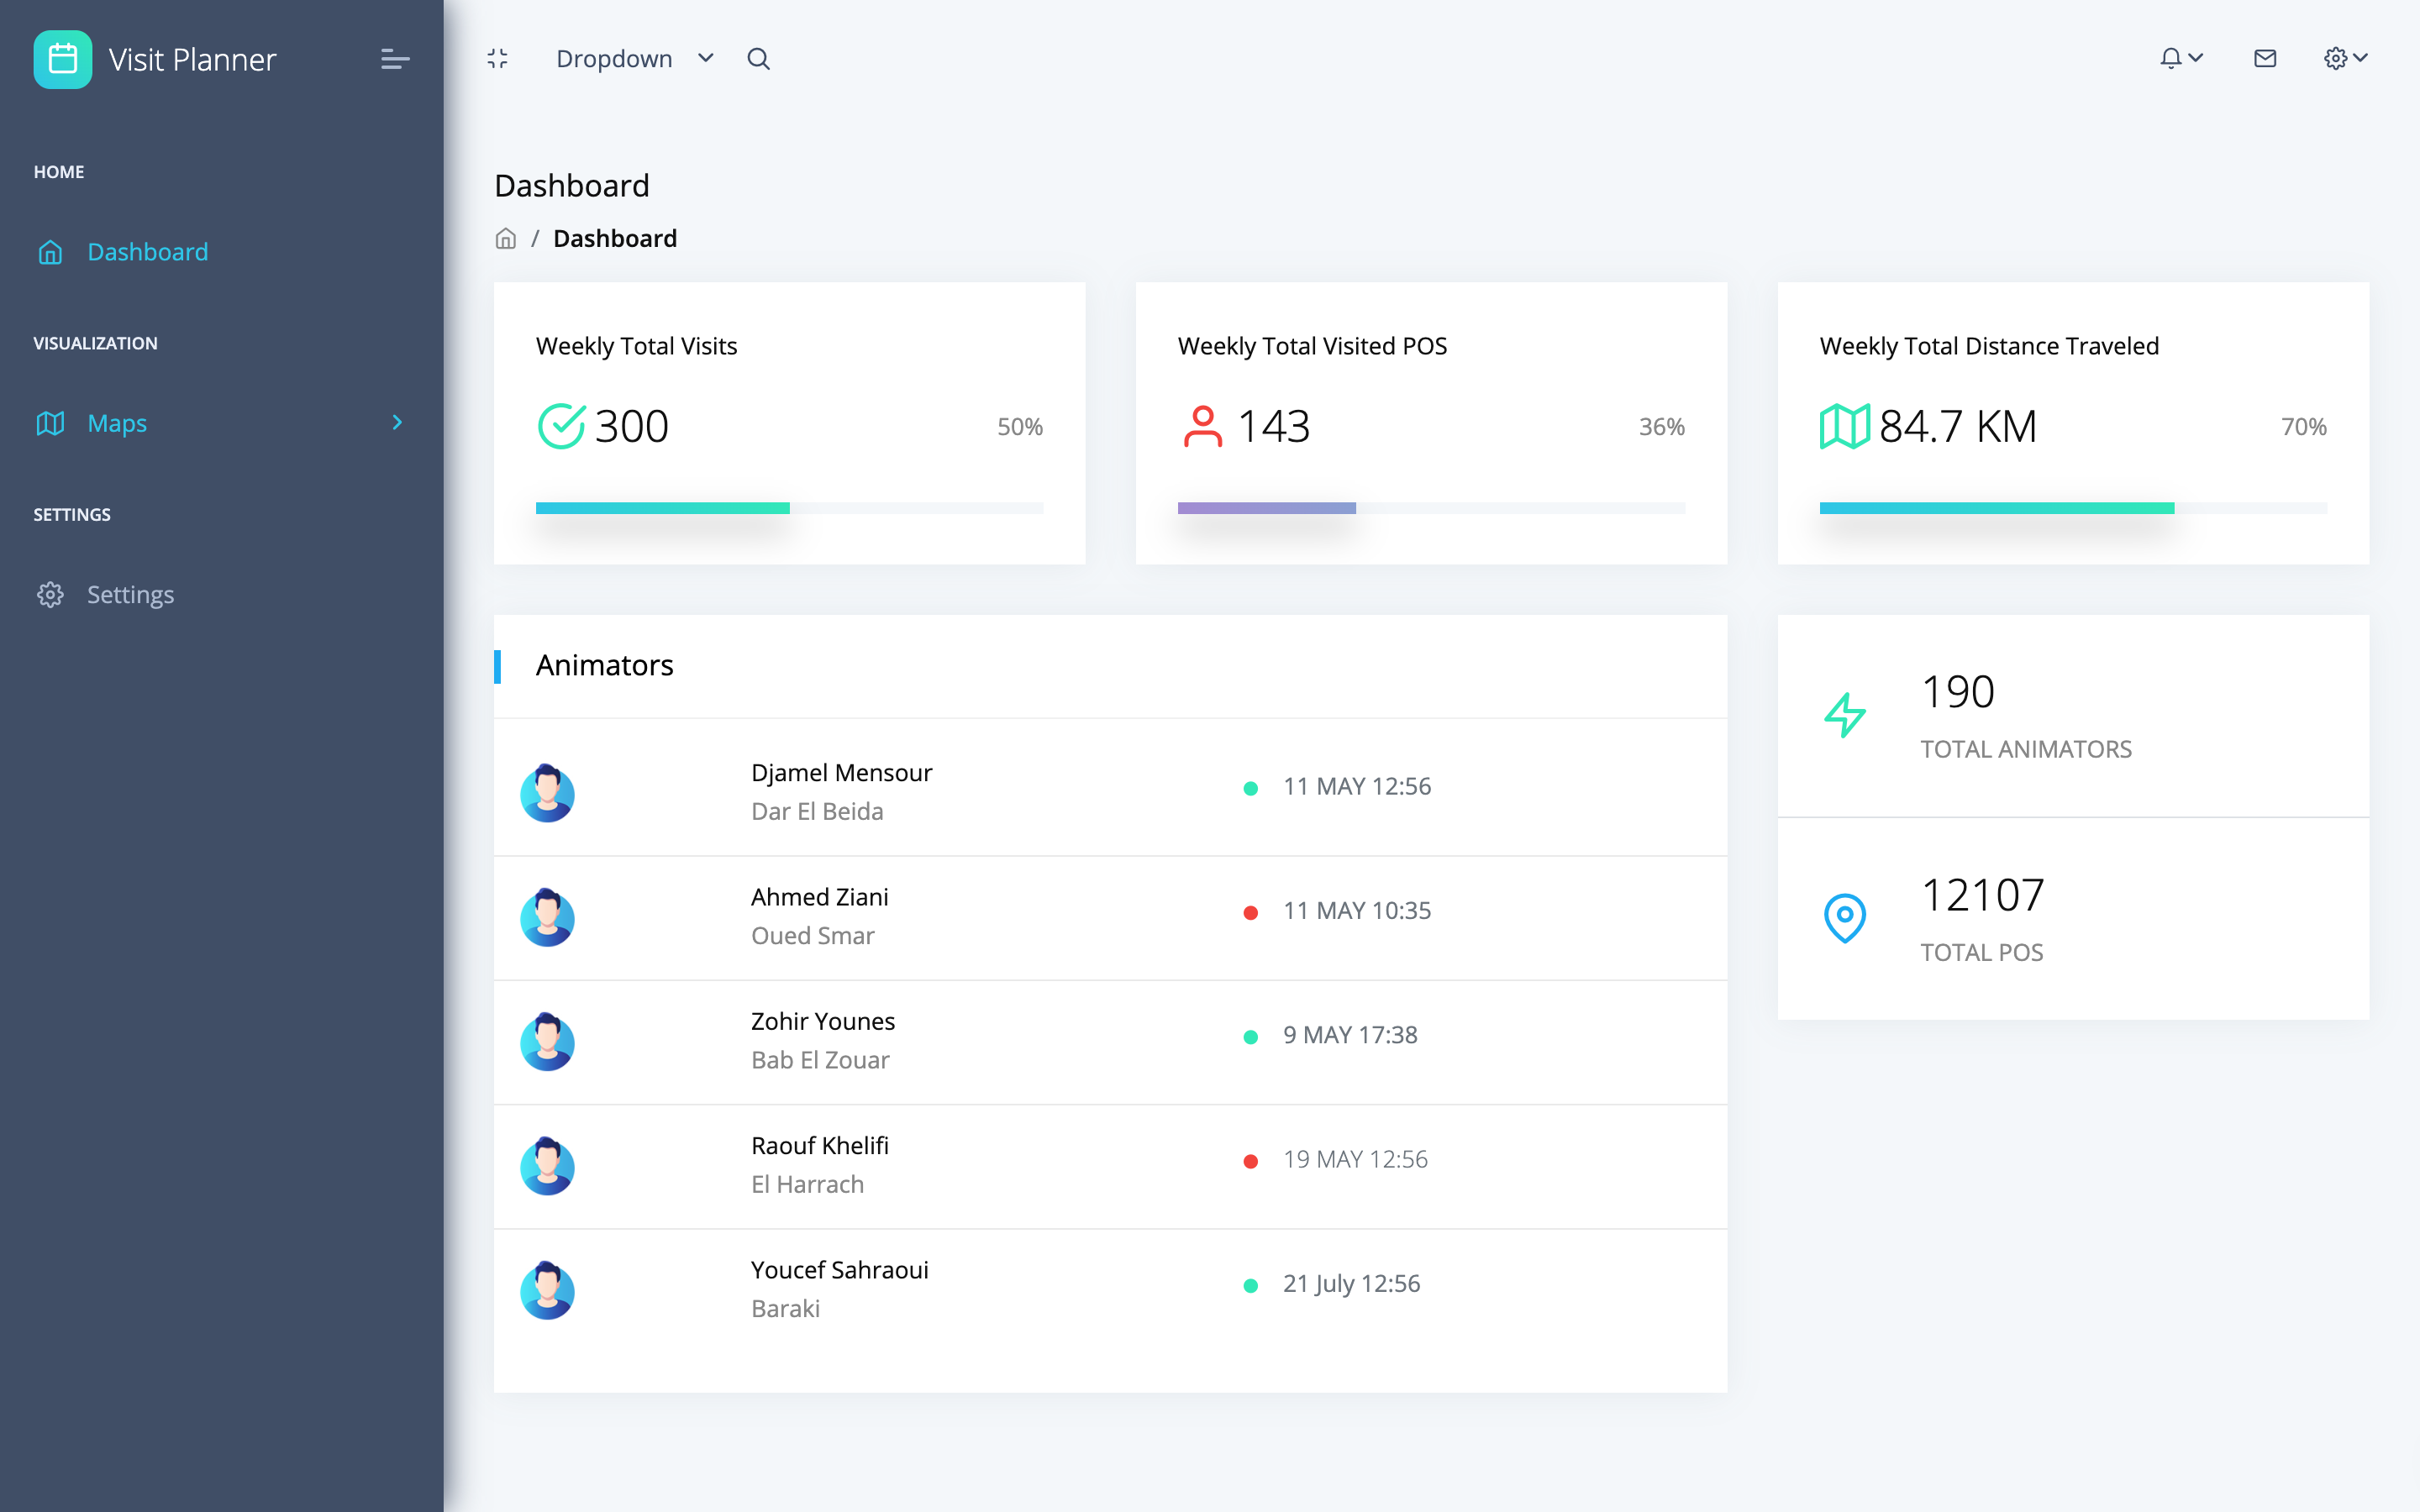
\includegraphics[width=15cm]{images_pfe/dashboard.png}
  \caption{Tableau de bord de la plateforme.}
  \label{fig:dashboard-page}
\end{figure}
\FloatBarrier

\begin{figure}[hbt!]
  \centering
  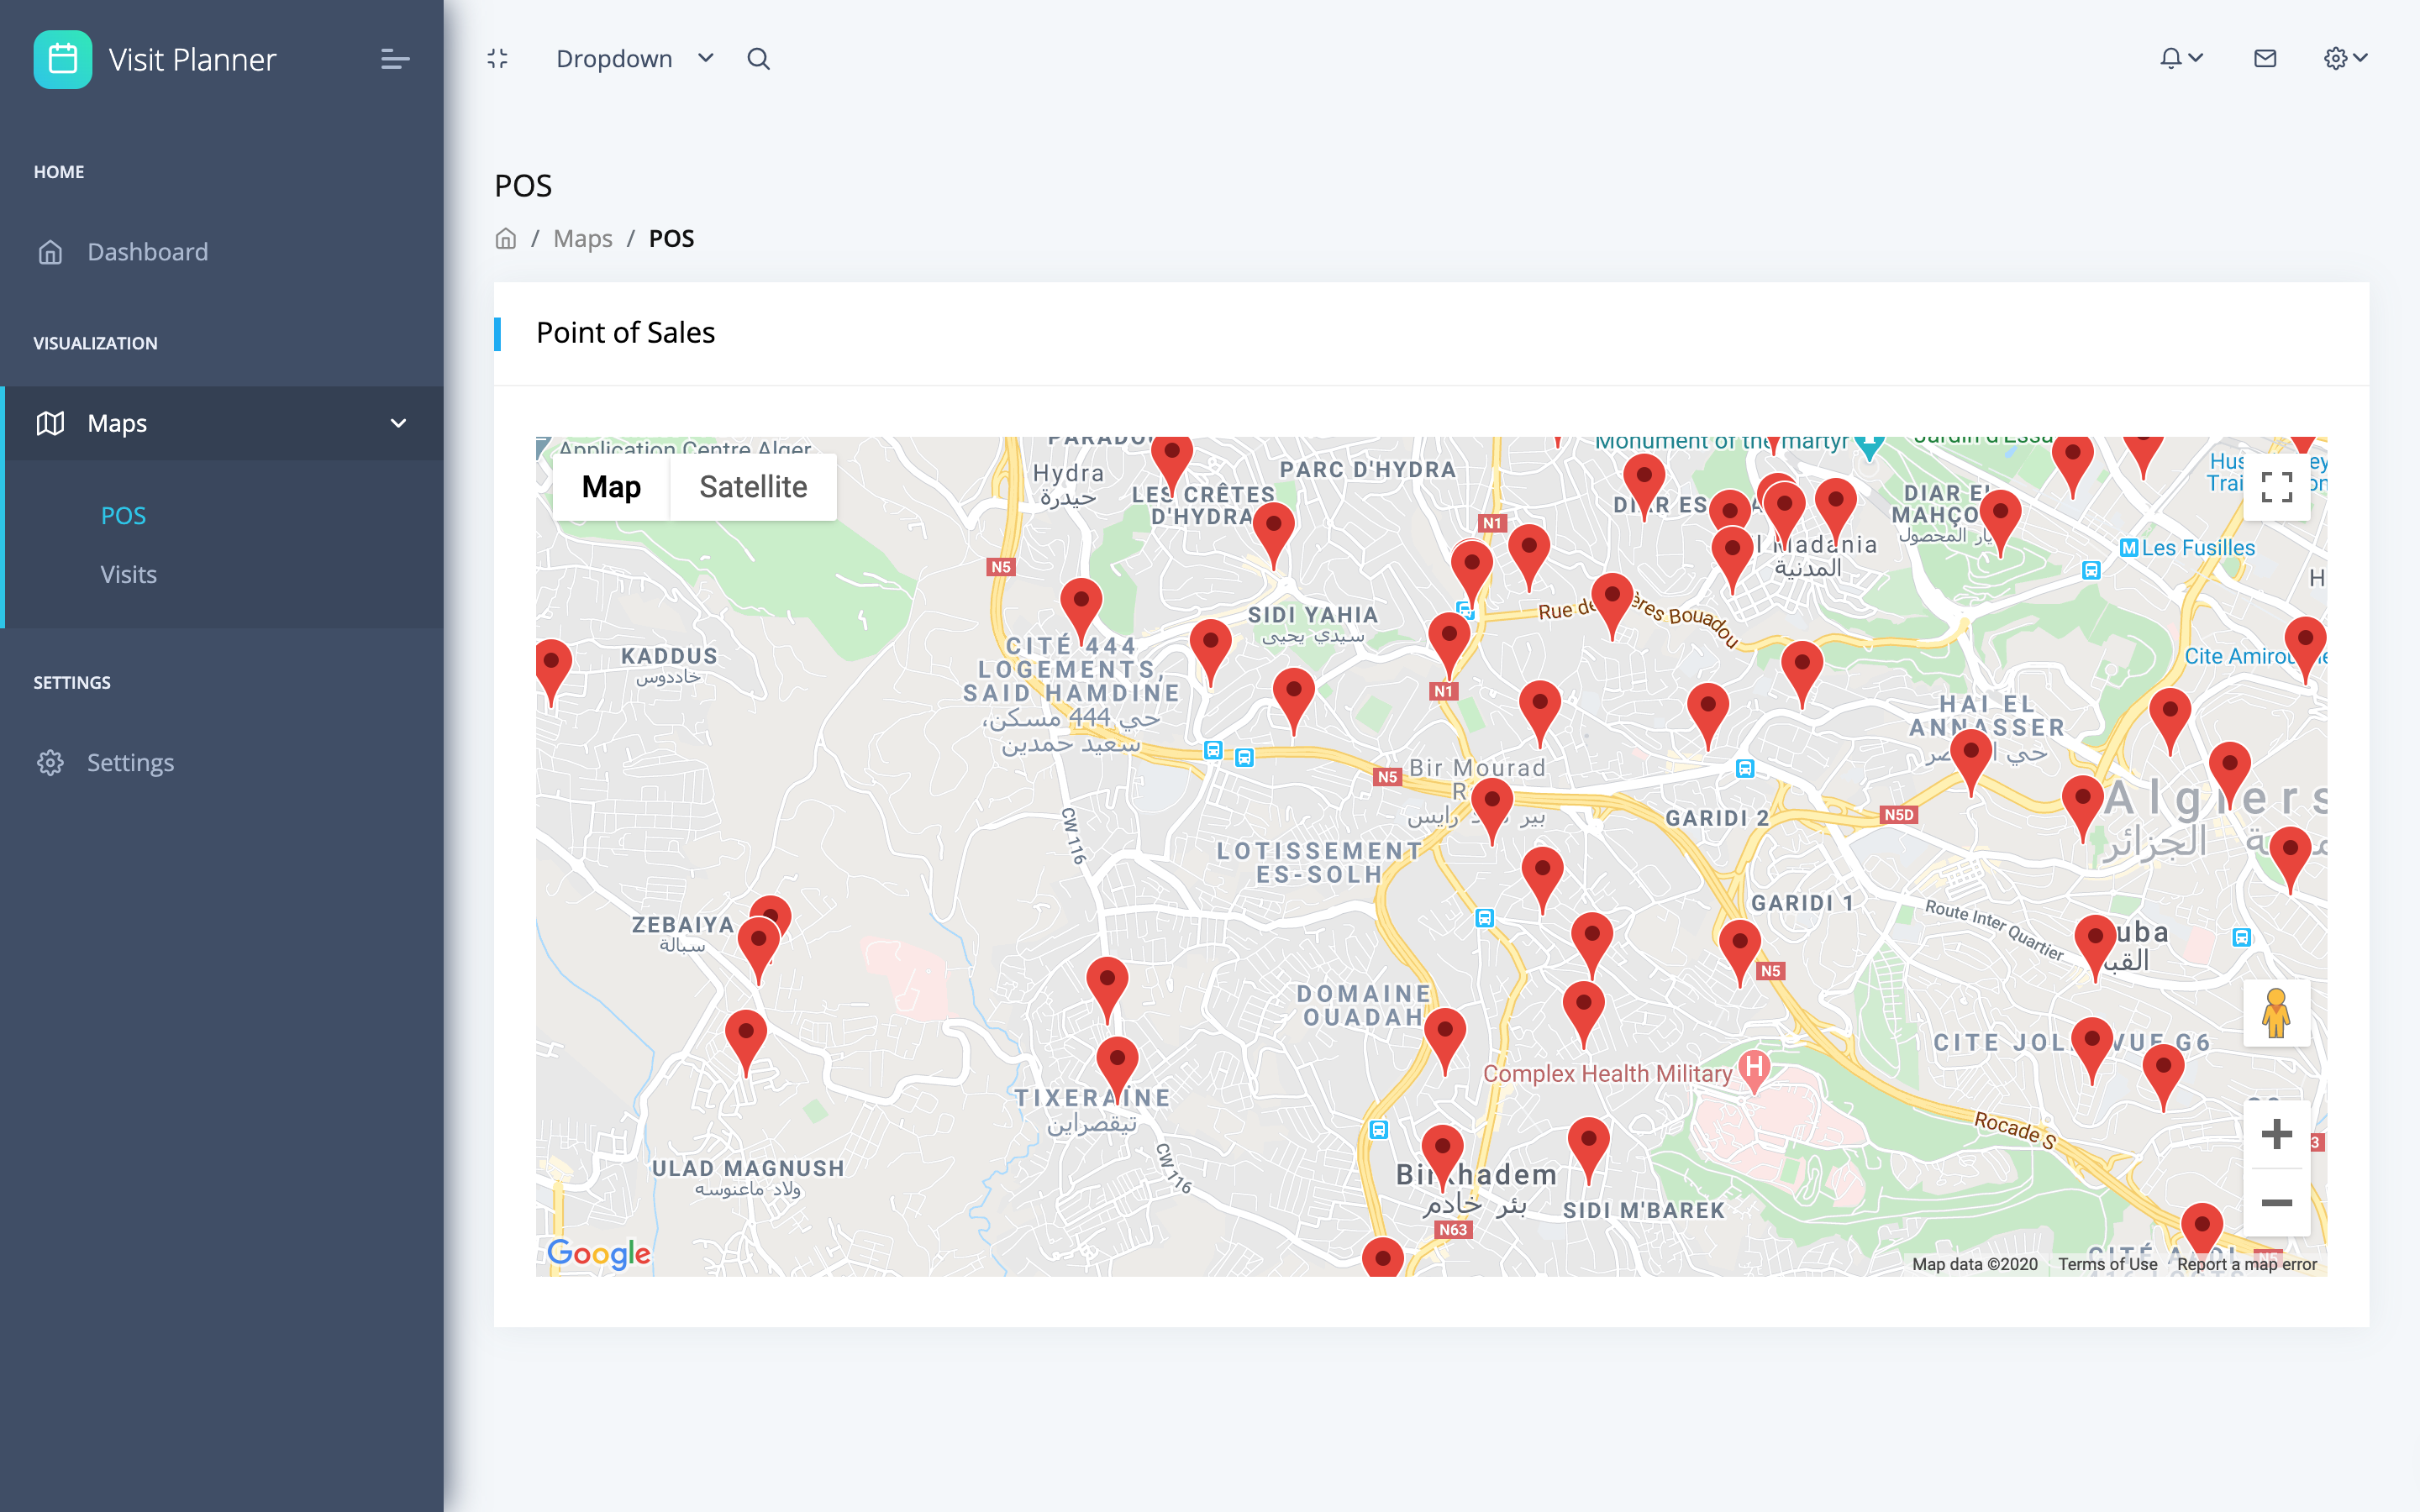
\includegraphics[width=15cm]{images_pfe/pos_visualization.png}
  \caption{Visualisation des points de vente.}
  \label{fig:pos-page}
\end{figure}
\FloatBarrier

Lorem ipsum dolor sit amet, consectetur adipiscing elit. Proin posuere euismod neque, non semper nibh viverra sed. Praesent ut varius magna. Fusce ipsum ante, semper nec interdum at, semper et lacus. Nulla ultrices magna a fringilla finibus. Etiam sollicitudin blandit ante. Vivamus blandit rhoncus tincidunt. Morbi sit amet congue purus. Praesent interdum gravida congue. Donec fermentum dui fermentum maximus rutrum. \textit{Visits} sous l'anglet \textit{Maps} toujours (Voir figure \ref{fig:routes-settings-page}). Lorem ipsum dolor sit amet, consectetur adipiscing elit. Proin posuere euismod neque, non semper nibh viverra sed. Praesent ut varius magna. Fusce ipsum ante, semper nec interdum at, semper et lacus. Nulla ultrices magna a fringilla finibus. Etiam sollicitudin blandit ante. Vivamus blandit rhoncus tincidunt. Morbi sit amet congue purus. Praesent interdum gravida congue. Donec fermentum dui fermentum maximus rutrum. \textit{Routes} (Voir figure \ref{fig:routes-visualization-page}). Lorem ipsum dolor sit amet, consectetur adipiscing elit. Proin posuere euismod neque, non semper nibh viverra sed. Praesent ut varius magna. Fusce ipsum ante, semper nec interdum at, semper et lacus. Nulla ultrices magna a fringilla finibus. Etiam sollicitudin blandit ante. Vivamus blandit rhoncus tincidunt. Morbi sit amet congue purus. Praesent interdum gravida congue. Donec fermentum dui fermentum maximus rutrum.e \textit{Settings} (Voir figure \ref{fig:general-settings-page}). L'animateur de son coté, peut visualiser la route de chaque jour du plan et synchroniser les routes en temps réel (Voir figure \ref{fig:routes-visualization-page}).


\begin{figure}[hbt!]
  \centering
  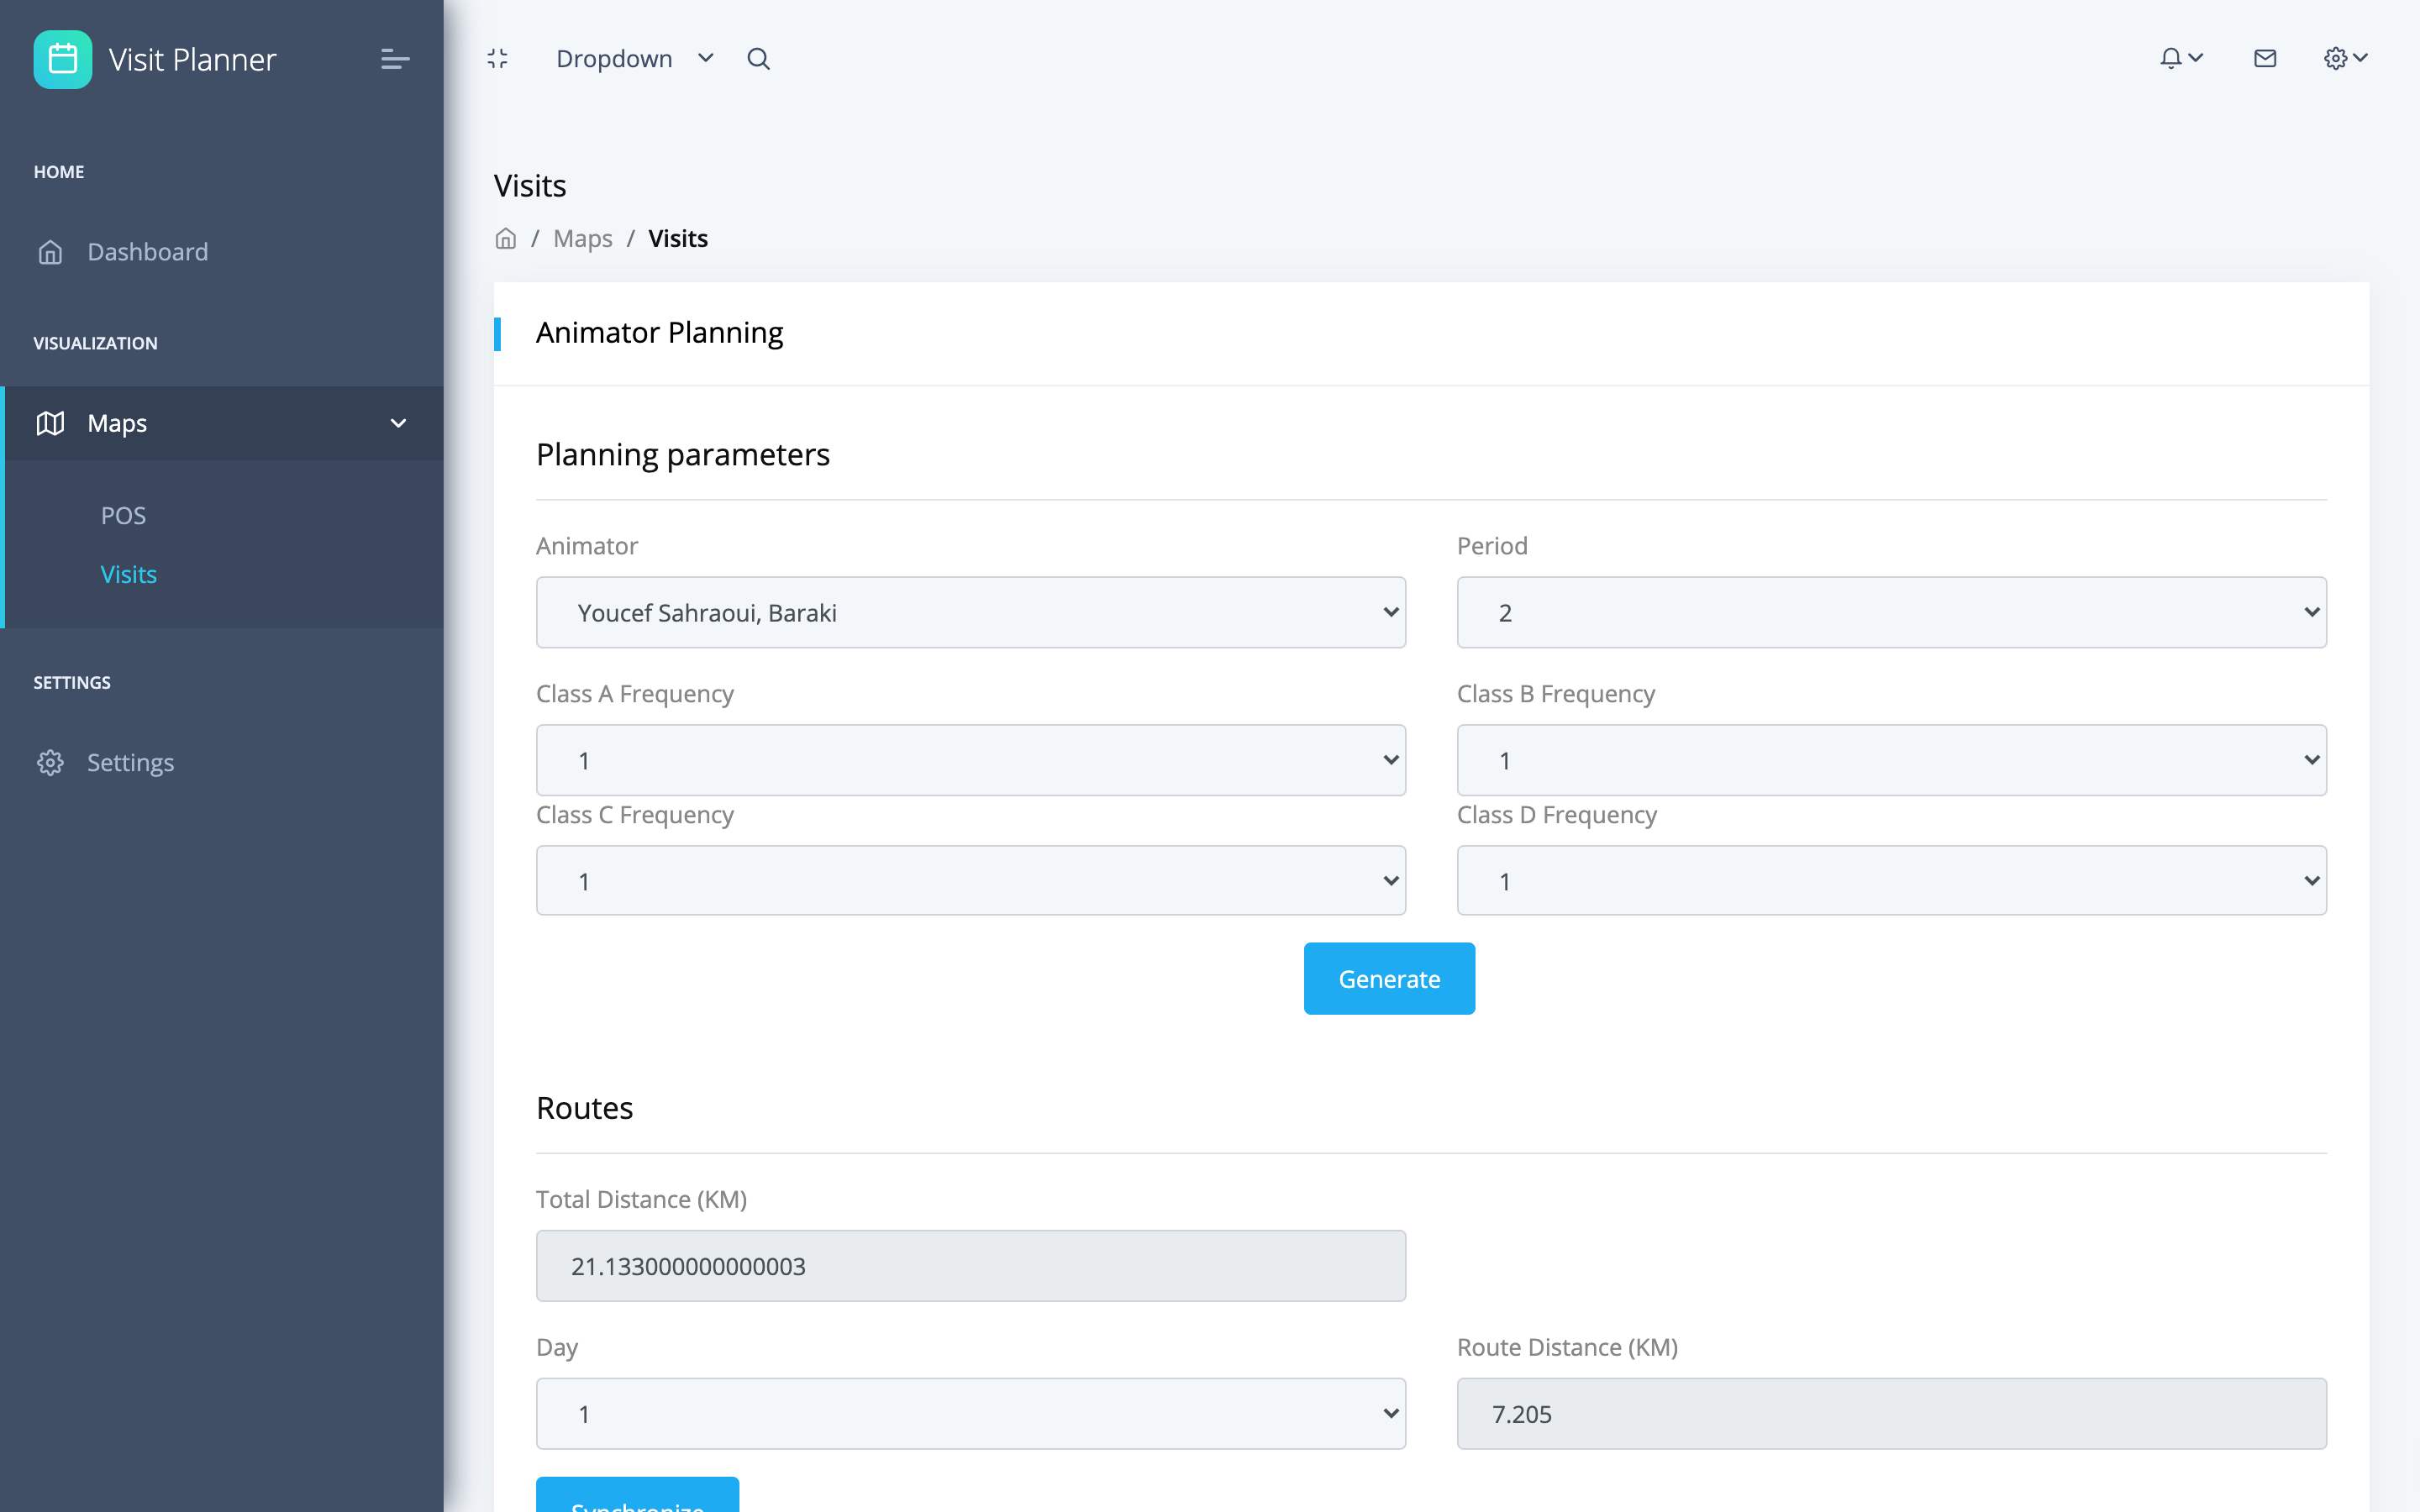
\includegraphics[width=15cm]{images_pfe/visites_settings.png}
  \caption{Paramétrage des visites.}
  \label{fig:routes-settings-page}
\end{figure}
\FloatBarrier


\begin{figure}[hbt!]
  \centering
  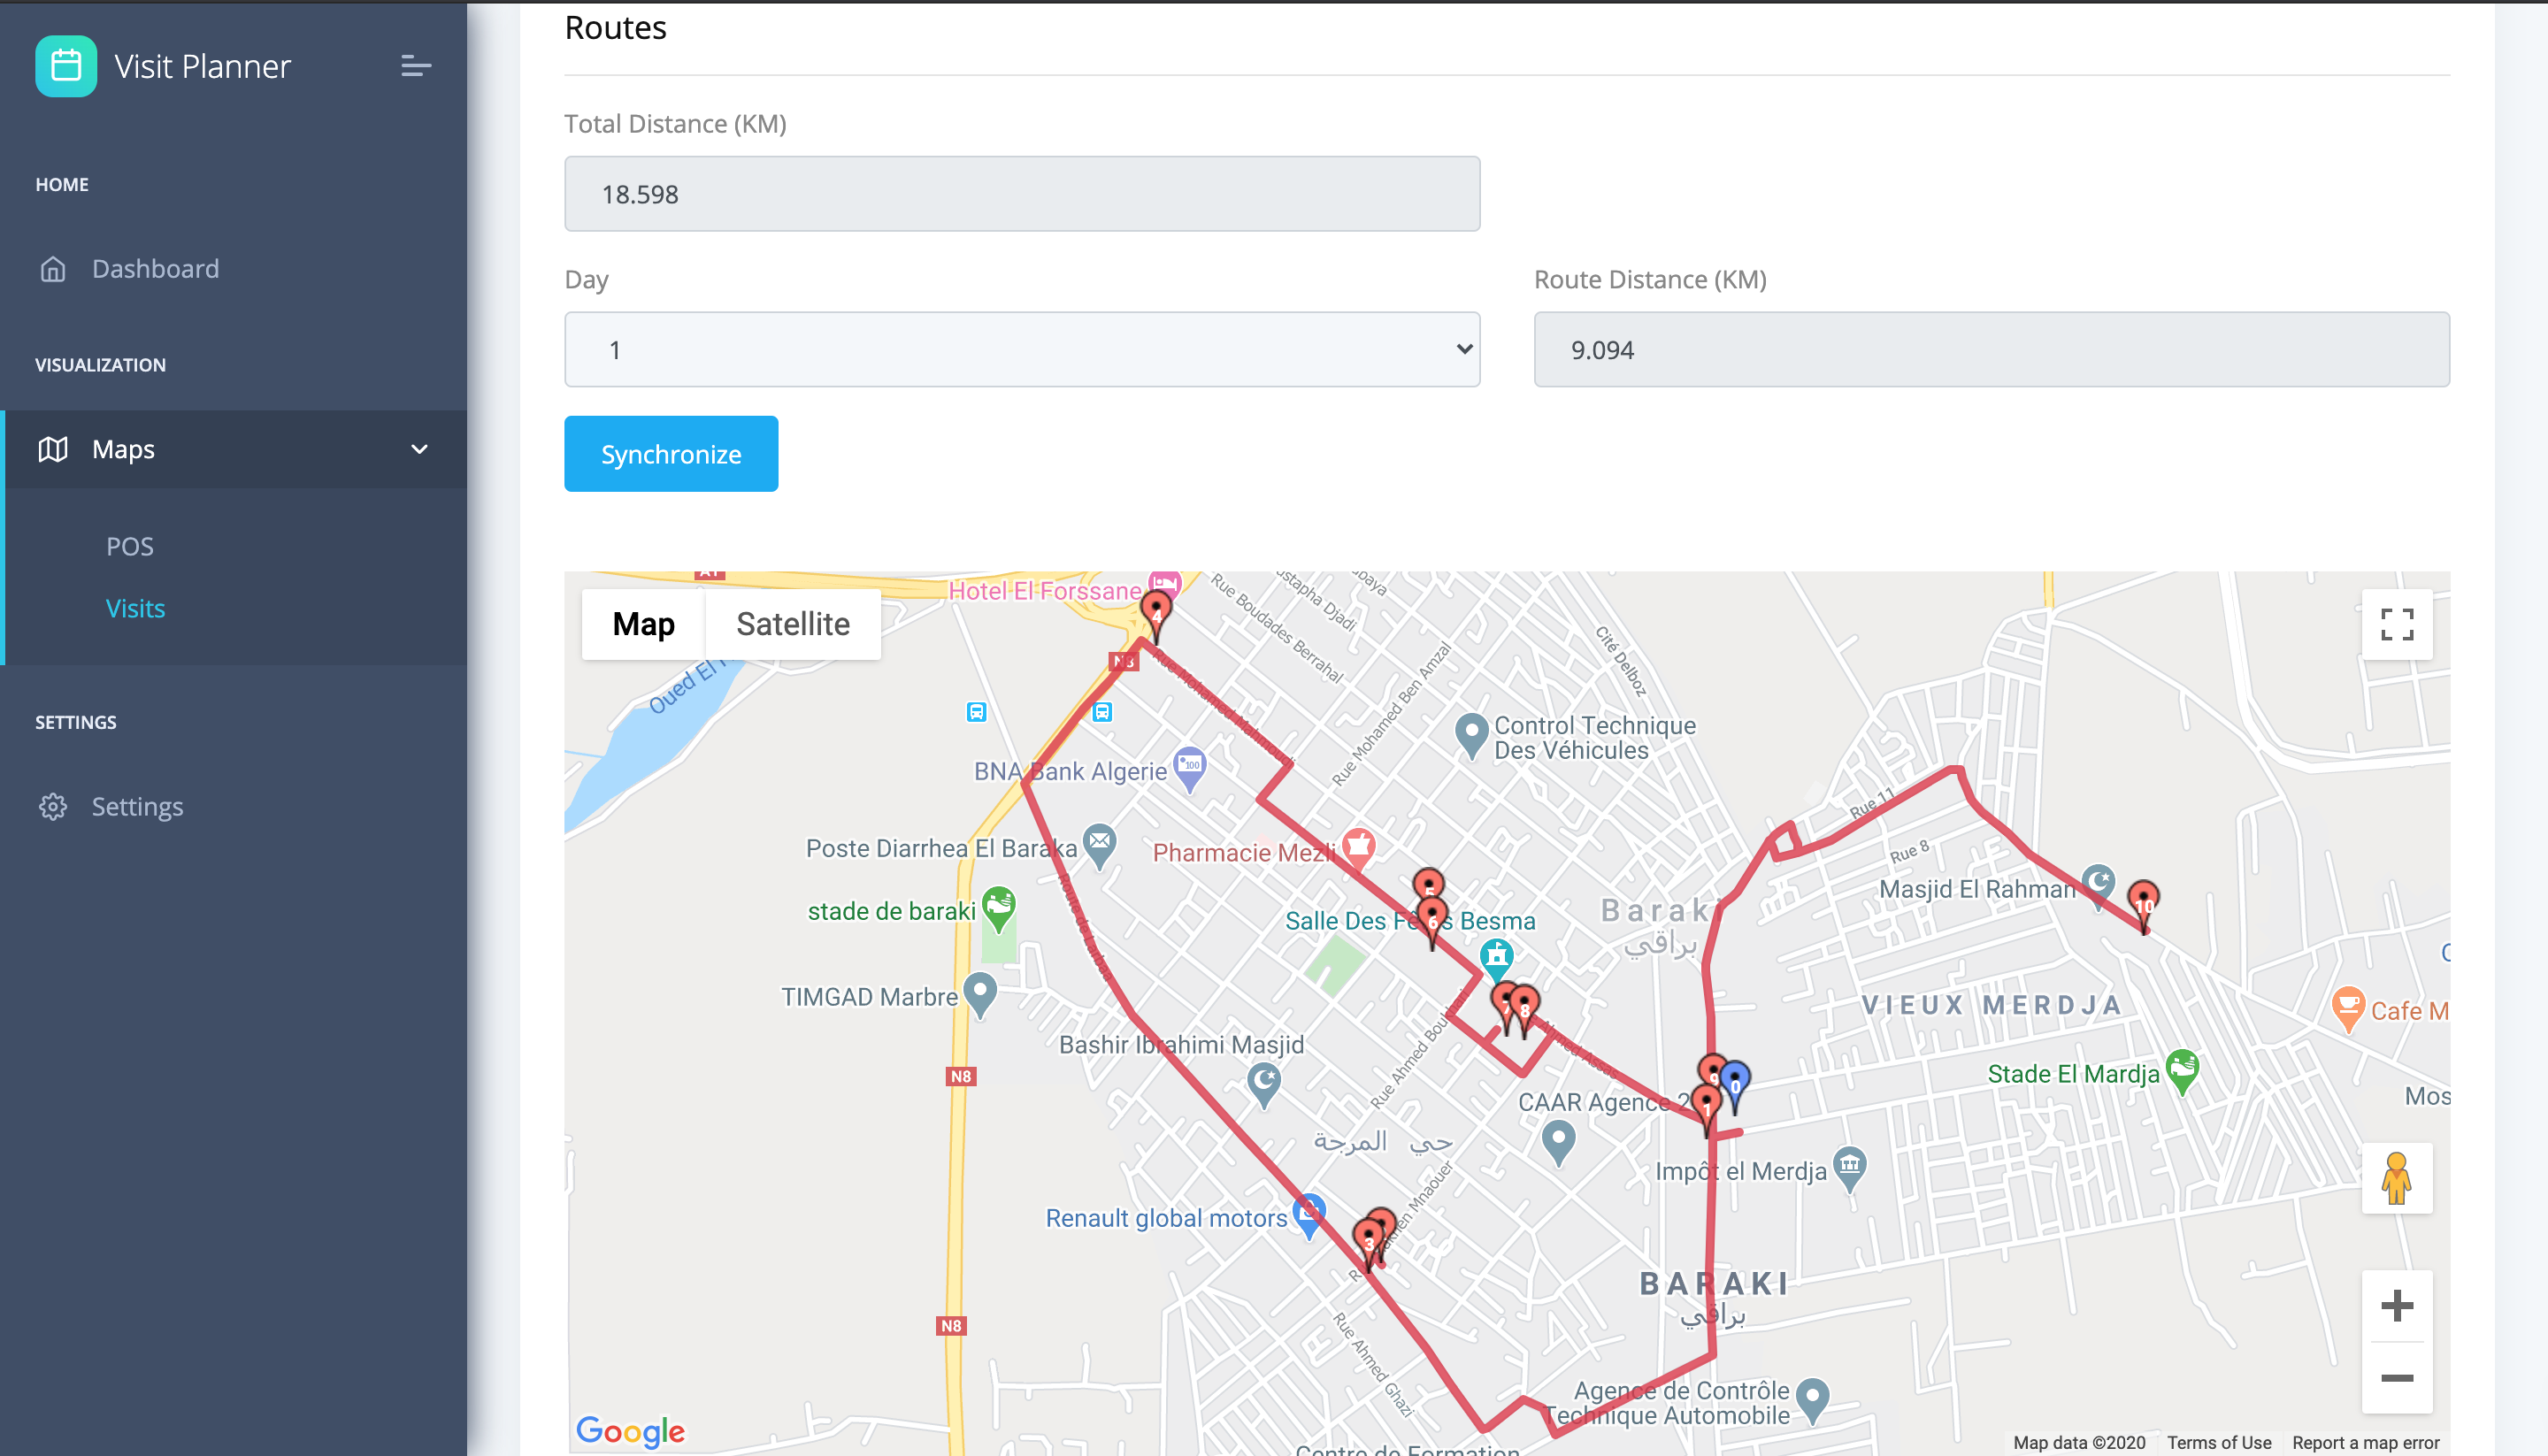
\includegraphics[width=15cm]{images_pfe/route_visualization.png}
  \caption{Visualisation des itinéraires.}
  \label{fig:routes-visualization-page}
\end{figure}
\FloatBarrier

\begin{figure}[hbt!]
  \centering
  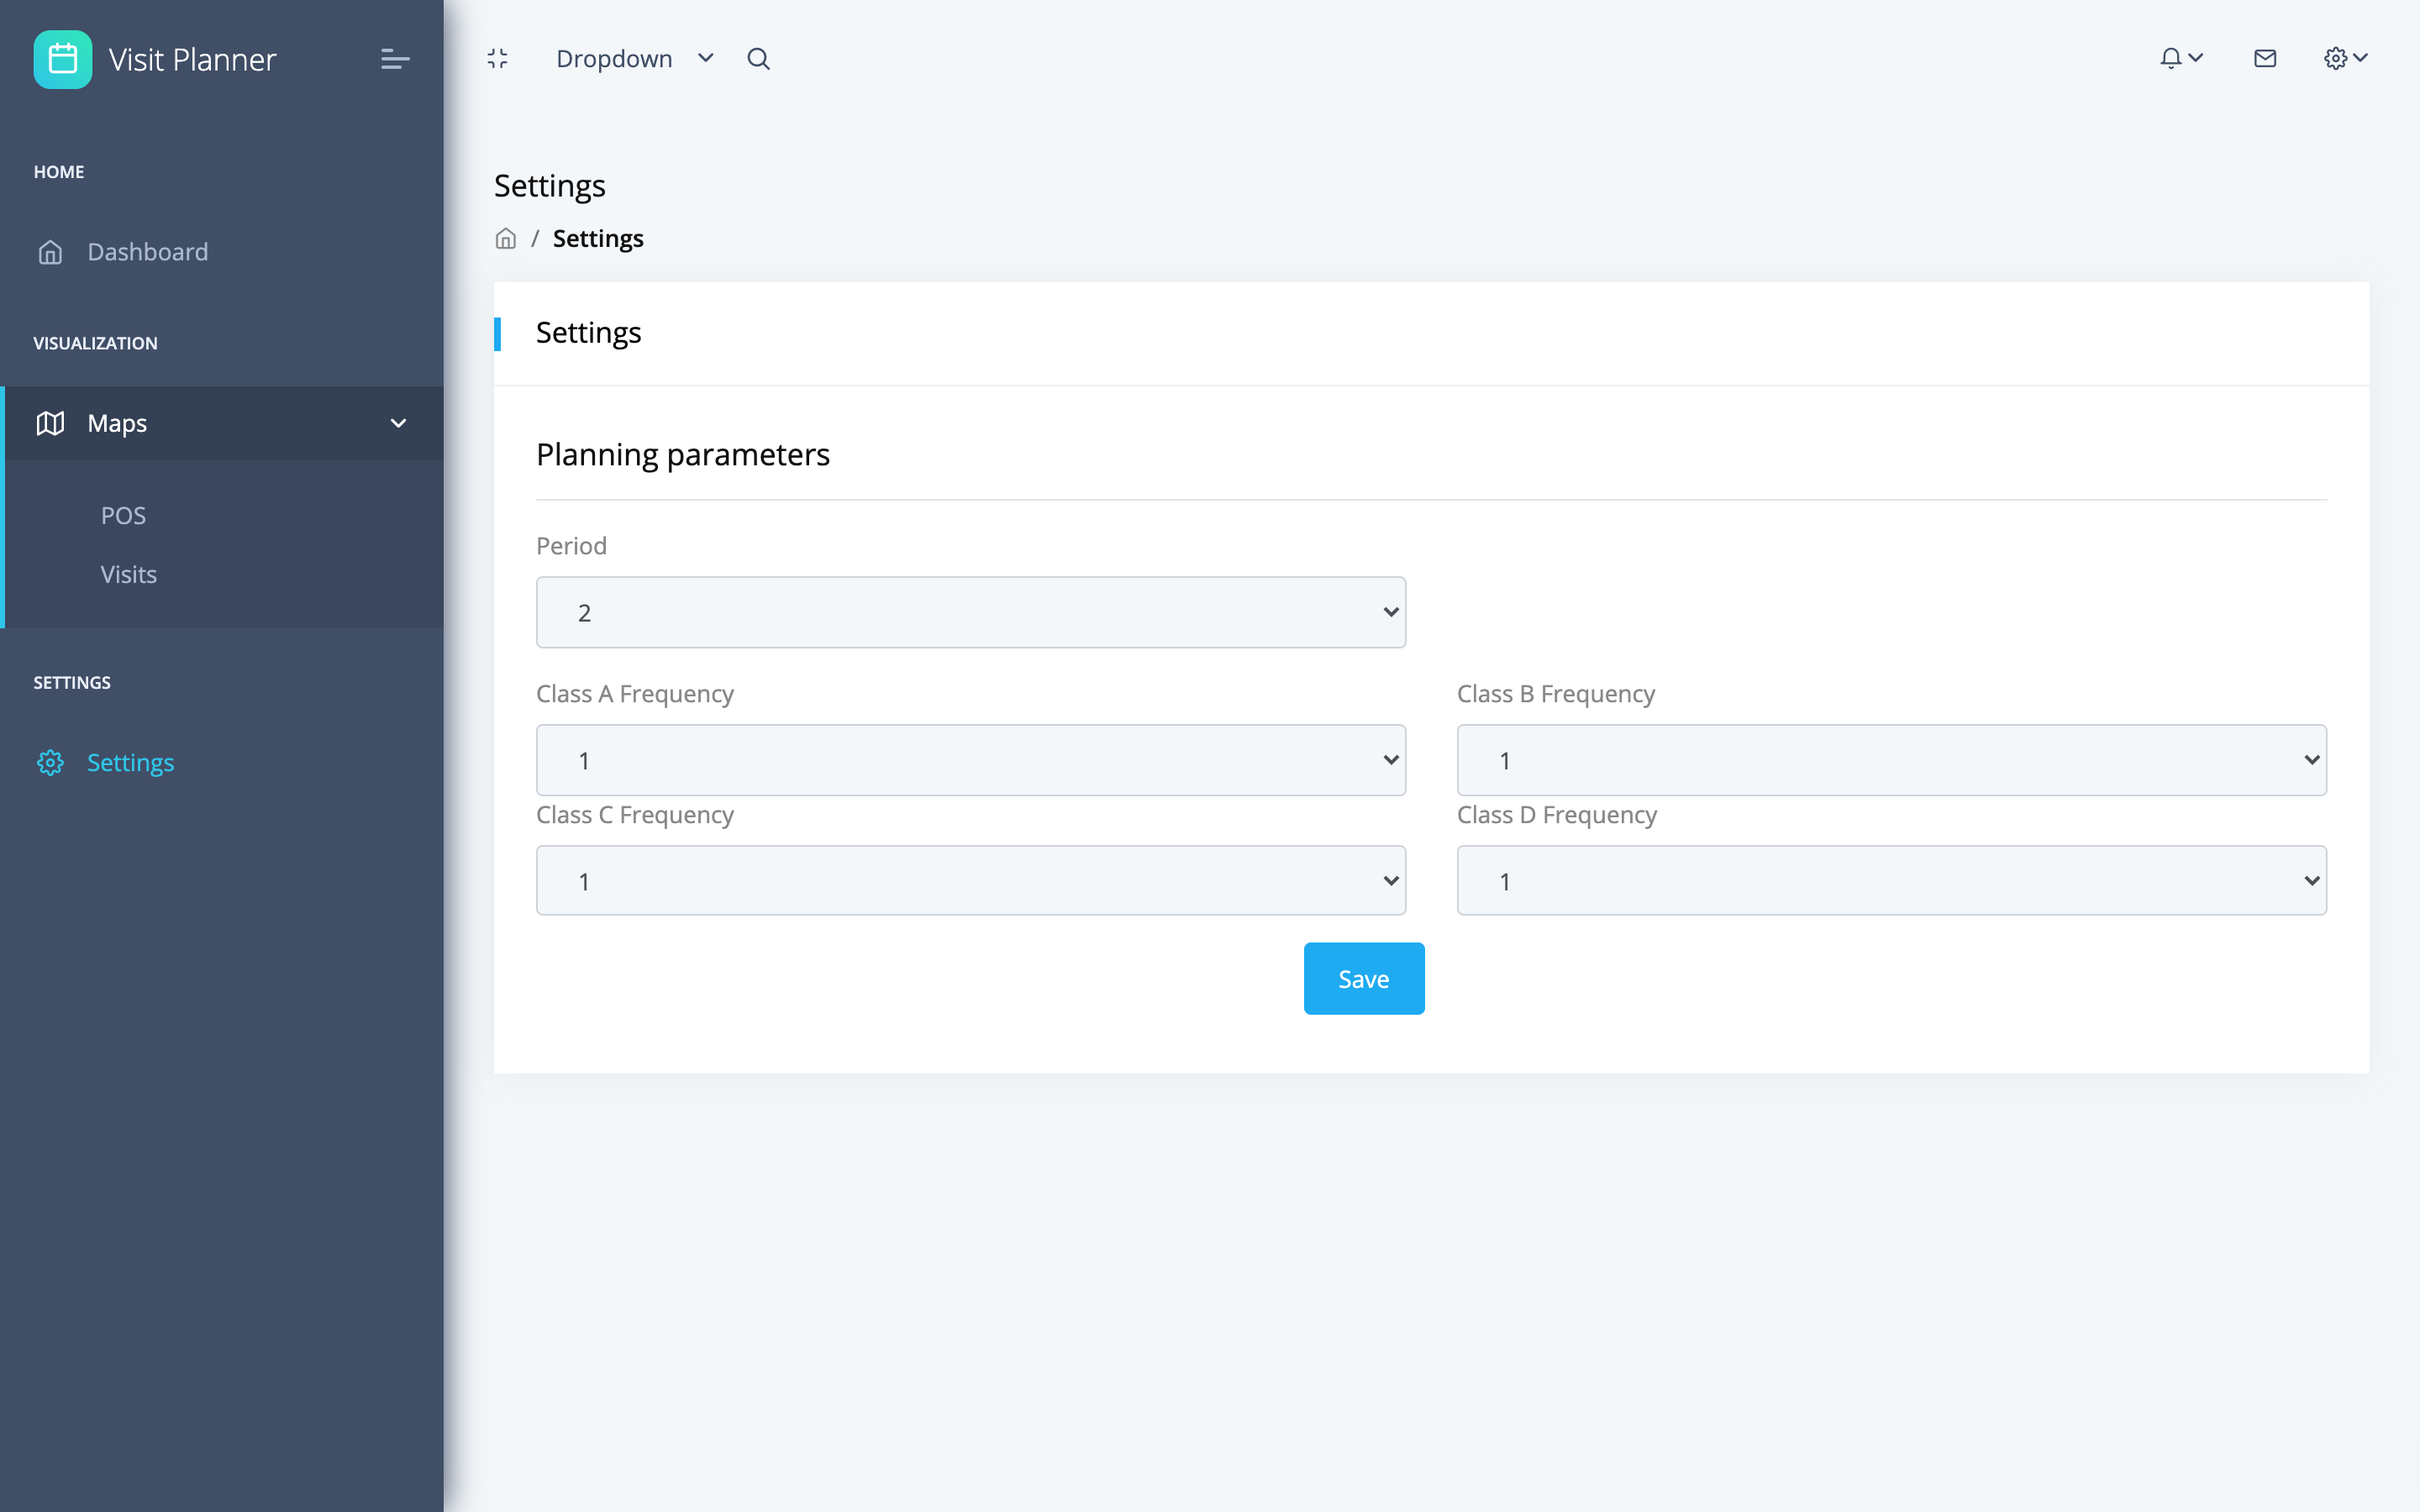
\includegraphics[width=15cm]{images_pfe/settings_page.png}
  \caption{Paramètres généraux.}
  \label{fig:general-settings-page}
\end{figure}
\FloatBarrier


\section{Conclusion}
Lorem ipsum dolor sit amet, consectetur adipiscing elit. Proin posuere euismod neque, non semper nibh viverra sed. Praesent ut varius magna. Fusce ipsum ante, semper nec interdum at, semper et lacus. Nulla ultrices magna a fringilla finibus. Etiam sollicitudin blandit ante. Vivamus blandit rhoncus tincidunt. Morbi sit amet congue purus. Praesent interdum gravida congue. Donec fermentum dui fermentum maximus rutrum.Lorem ipsum dolor sit amet, consectetur adipiscing elit. Proin posuere euismod neque, non semper nibh viverra sed. Praesent ut varius magna. Fusce ipsum ante, semper nec interdum at, semper et lacus. Nulla ultrices magna a fringilla finibus. Etiam sollicitudin blandit ante. Vivamus blandit rhoncus tincidunt. Morbi sit amet congue purus. Praesent interdum gravida congue. Donec fermentum dui fermentum maximus rutrum.




